


\setcounter{chapter}{1}


\chapter{子群}

\section{定义和例子}

揭示由一组公理定义的任何数学对象的结构的一个基本方法是研究该对象中同样满足这些公理的子集。
我们从讨论群的子群开始这个计划。
揭示结构的第二个基本方法是研究对象的商；商群的概念（粗略地说是一种将一个群坍缩成一个更小的群的方法）将在下一章讨论。
这两个主题将在全文中反复出现，当我们研究群的子群和商群、环的子环和商环、向量空间的子空间和商空间等时。

\begin{definition}
设 \( G \) 是一个群。
\( G \) 的子集 \( H \) 称为 \( G \) 的\textbf{子群}，如果 \( H \) 非空，并且 \( H \) 在乘积和逆下封闭（即 \( x, y \in H \) 蕴含 \( x^{-1} \in H \) 且 \( xy \in H \)）. 
如果 \( H \) 是 \( G \) 的子群，我们记作 \( H \leq G \).
\end{definition}

\( G \) 的子群正是这样的子集：它们自身关于 \( G \) 中定义的运算构成群，即 \( G \) 上的二元运算限制到 \( H \) 上给出一个二元运算，该运算是结合的，在 \( H \) 中有单位元，并且 \( H \) 中每个元素在 \( H \) 中有逆元。

当我们说 \( H \) 是 \( G \) 的子群时，我们总是指 \( H \) 的运算是 \( G \) 的运算限制到 \( H \) 上（一般情况下，子集 \( H \) 可能关于某个不同于 \( G \) 限制运算的运算构成群，参见后面的例 \ref{exa:2.1}(5)(a)）. 
像我们对函数限制到子集所做的那样，我们将用相同的符号表示 \( G \) 的运算和子群 \( H \) 的运算。
如果 \( H \leq G \) 且 \( H \neq G \)，我们记作 \( H < G \) 以强调包含是严格的。

如果 \( H \) 是 \( G \) 的子群，那么由于 \( H \) 的运算是 \( G \) 的运算限制到 \( H \) 上，子群 \( H \) 中的任何方程也可以看作群 \( G \) 中的方程。
因此 \( G \) 中的消去律意味着 \( H \) 的单位元与 \( G \) 的单位元相同（特别地，每个子群必须包含 \( 1 \)，即 \( G \) 的单位元），并且 \( H \) 中元素 \( x \) 的逆元与 \( x \) 作为 \( G \) 中元素时的逆元相同（所以记号 \( x^{-1} \) 是明确的）。

\begin{example}\label{exa:2.1}
\begin{enumerate}[label=(\arabic*)]
\item \(\mathbb{Z} \leq \mathbb{Q}\) 且 \(\mathbb{Q} \leq \mathbb{R}\)，运算为加法。

\item 任何群 \( G \) 有两个子群：\( H = G \) 和 \( H = \{1\} \)；后者称为\textbf{平凡子群}，以后记作 1.

\item 若 \( G = D_{2n} \) 是 \( 2n \) 阶二面体群，令 \( H = \{1, r, r^2, \ldots, r^{n-1}\} \)，即 \( G \) 中所有旋转的集合。
由于两个旋转的乘积仍是旋转，旋转的逆也是旋转，故 \( H \) 是 \( D_{2n} \) 的一个 \( n \) 阶子群。

\item 偶数集合是整数加法群的一个子群。

\item 一些不是子群的子集例子：
\begin{enumerate}
\item \(\mathbb{Q} - \{0\}\) 在乘法下不是 \(\mathbb{R}\) 在加法下的子群，尽管两者都是群且 \(\mathbb{Q} - \{0\}\) 是 \(\mathbb{R}\) 的子集；%这是因为
\(\mathbb{Q} - \{0\}\) 上的乘法不是 \(\mathbb{R}\) 上加法的限制。
\item \(\mathbb{Z}^+\)（在加法下）不是 \(\mathbb{Z}\)（在加法下）的子群，因为尽管 \(\mathbb{Z}^+\) 在加法下封闭，但它不包含 \(\mathbb{Z}\) 的单位元 \(0\)，
并且尽管每个 \(x \in \mathbb{Z}^+\) 在 \(\mathbb{Z}\) 中有加法逆元 \(-x\)，但 \(-x \notin \mathbb{Z}^+\)，即 \(\mathbb{Z}^+\) 在取逆运算下不封闭（特别地，\(\mathbb{Z}^+\) 在加法下不是群）。
类似地，\((\mathbb{Z} - \{0\}, \times)\) 不是 \((\mathbb{Q} - \{0\}, \times)\) 的子群。
\item \(D_6\) 不是 \(D_8\) 的子群，因为前者甚至不是后者的子集。
\end{enumerate}

\item “是子群”关系是传递的：若 \( H \) 是群 \( G \) 的子群，且 \( K \) 是 \( H \) 的子群，则 \( K \) 也是 \( G \) 的子群。
\end{enumerate}
\end{example}

正如我们在第 1 章所见，即使对于简单的例子，验证任何给定二元运算的所有群公理（尤其是结合律）也可能十分繁琐。
然而，一旦我们知道了一个群，检查它的一个子集是否是子群就容易得多了，因为只需检查乘法和取逆下的封闭性。
下面的命题表明这两者可以合并为一个检验，同时还表明对于有限群，只需检查乘法封闭性即可。

\begin{proposition}[\textbf{子群判别法}]
群 \( G \) 的子集 \( H \) 是子群当且仅当
\begin{enumerate}[label=(\arabic*)]
\item \( H \neq \emptyset \)，且
\item 对所有 \( x, y \in H \)，有 \( xy^{-1} \in H \).
\end{enumerate}
此外，若 \( H \) 是有限的，则只需检查 \( H \) 非空且在乘法下封闭。
\end{proposition}

\begin{proof}
若 \( H \) 是 \( G \) 的子群，则显然 (1) 和 (2) 成立，因为 \( H \) 包含 \( G \) 的单位元及每个元素的逆元，并且 \( H \) 在乘法下封闭。

反之，假设 \( H \) 满足 (1) 和 (2). 
取任意 \( x \in H \)（由 (1) 存在）。
令 \( y = x \)，应用 (2) 得 \( 1 = xx^{-1} \in H \)，所以 \( H \) 包含 \( G \) 的单位元。
然后，再次由 (2)，因 \( H \) 包含 1 和 \( x \)，\( H \) 包含元素 \( 1x^{-1} \)，即 \( x^{-1} \in H \)，所以 \( H \) 在取逆下封闭。
%左脚踩右脚上天这一块./
最后，若 \( x, y \in H \)，则由已证结果 \( y^{-1} \in H \)，再由 (2) 得 \( x(y^{-1})^{-1} = xy \in H \)。
故 \( H \) 也在乘法下封闭，从而 \( H \) 是 \( G \) 的子群。

现在假设 \( H \) 是有限的且在乘法下封闭，并令 \( x \) 为 \( H \) 中的任意元素。
则 \( x, x^2, x^3, \ldots \) 中只有有限多个不同的元素，因此对某些整数 \( a, b \)（\( b > a \)）有 \( x^a = x^b \). 若 \( n = b - a \)，则 \( x^n = 1 \)，所以特别地，\( H \) 中每个元素都是有限阶的。
于是 \( x^{n-1} = x^{-1} \) 是 \( H \) 中的元素，因此 \( H \) 自动在取逆下也封闭。
\end{proof}


\subsection*{习题}
设G是一个群。
\begin{enumerate}
\item 在 (a)-(e) 中证明指定的子集是给定群的子群：
\begin{enumerate}[label=(\alph*)]
\item 形如 \( a + ai \)（\( a \in \mathbb{R} \)）的复数集合（加法下）；
\item 绝对值为 1 的复数集合，即复平面上的单位圆（乘法下）；
\item 固定 \( n \in \mathbb{Z}^+ \)，分母整除 \( n \) 的有理数集合（加法下）；
\item 固定 \( n \in \mathbb{Z}^+ \)，分母与 \( n \) 互质的有理数集合（加法下）；
%哇还有B站视频《只有有限个素数的整环》
\item 平方为有理数的非零实数集合（乘法下）。
\end{enumerate}

\item 在 (a)-(e) 中证明指定的子集不是给定群的子群：
\begin{enumerate}[label=(\alph*)]
\item \( S_n \)（\( n \geq 3 \)）中对换的集合；
\item \( D_{2n} \)（\( n \geq 3 \)）中反射的集合；
\item 对合数 \( n > 1 \) 和包含 \( n \) 阶元的群 \( G \)，集合
\(
\{ x \in G \mid |x| = n \} \cup \{ 1 \};
\)
\item \( \mathbb{Z} \) 中正负奇数与 0 一起的集合；
\item 平方为有理数的实数集合（加法下）。
\end{enumerate}

\item 证明二面体群 \( D_8 \) 的下列子集实际上是子群：
\begin{enumerate}[label=(\alph*)]
\item \( \{ 1, r^2, s, sr^2 \} \)；
\item \( \{ 1, r^2, sr, sr^3 \} \).
\end{enumerate}

\item 给出一个具体例子：群 \( G \) 及其无限子集 \( H \)，使得 \( H \) 在群运算下封闭但不是 \( G \) 的子群。

\item 证明 \( G \) 不可能有一个阶为 \( n-1 \) 的子群 \( H \)，其中 \( n = |G| > 2 \).

\item 设 \( G \) 是阿贝尔群。证明 \( \{ g \in G \mid |g| < \infty \} \) 是 \( G \) 的子群（称为 \( G \) 的\textbf{挠子群}）。
给出一个具体例子说明当 \( G \) 非阿贝尔时这个集合可能不是子群。

\item 固定 \( n \in \mathbb{Z} \) 且 \( n > 1 \). 求 \( \mathbb{Z} \times (\mathbb{Z}/n\mathbb{Z}) \) 的挠子群（见上一题）。
证明无限阶元素与单位元一起的集合不是这个直积的子群。

\item 设 \( H \) 和 \( K \) 是 \( G \) 的子群。证明 \( H \cup K \) 是子群当且仅当 \( H \subseteq K \) 或 \( K \subseteq H \).

\item 设 \( G = GL_n(F) \)，其中 \( F \) 是任意域。定义
\[
SL_n(F) = \{ A \in GL_n(F) \mid \det(A) = 1 \}
\]
（称为\textbf{特殊线性群}）。
证明 \( SL_n(F) \leq GL_n(F) \).

\item \begin{enumerate}[label=(\alph*)]
\item 证明若 \( H \) 和 \( K \) 是 \( G \) 的子群，则它们的交集 \( H \cap K \) 也是子群。
\item 证明 \( G \) 的任意非空子群族（不必可数）的交仍然是 \( G \) 的子群。
\end{enumerate}

\item 设 \( A \) 和 \( B \) 是群。
证明下列集合是直积 \( A \times B \) 的子群：
\begin{enumerate}[label=(\alph*)]
\item \( \{ (a, 1) \mid a \in A \} \)；
\item \( \{ (1, b) \mid b \in B \} \)；
\item 当 \( A = B \) 且运算相同时，\( \{ (a, b) \in A \times B \mid a = b \} \)（称为\textbf{对角子群}）。
\end{enumerate}

\item 设 \( A \) 是阿贝尔群，并固定某个 \( n \in \mathbb{Z} \). 
证明下列集合是 \( A \) 的子群：
\begin{enumerate}[label=(\alph*)]
\item \( \{a^n \mid a \in A\} \)；
\item \( \{a \in A \mid a^n = 1\} \).
\end{enumerate}

\item 设 \( H \) 是有理数加法群的子群，具有性质：对每个非零元素 \( x \in H \)，有 \( 1/x \in H \). 证明 \( H = 0 \) 或 \( H = \mathbb{Q} \).

\item 证明 \( \{x \in D_{2n} \mid x^2 = 1\} \) 不是 \( D_{2n} \) 的子群（这里 \( n \geq 3 \)）.

\item 设 \( H_1 \leq H_2 \leq \cdots \) 是 \( G \) 的一个上升子群链。
证明 \( \bigcup_{i=1}^{\infty} H_i \) 是 \( G \) 的子群。

\item 设 \( n \in \mathbb{Z}^+ \)，\( F \) 是域。
证明集合
\(
\{(a_{ij}) \in GL_n(F) \mid a_{ij} = 0 \text{ 对所有 } i > j\}
\)
是 \( GL_n(F) \) 的子群（称为\textbf{上三角矩阵群}）。

\item 设 \( n \in \mathbb{Z}^+ \)，\( F \) 是域。
证明集合
\(
\{(a_{ij}) \in GL_n(F) \mid a_{ij} = 0 \text{ 对所有 } i > j,\ \text{且 } a_{ii} = 1 \text{ 对所有 } i\}
\)
是 \( GL_n(F) \) 的子群。
\end{enumerate}


\section{中心化子与正规化子，稳定子与核}

我们现在引入任意群 \( G \) 的一些重要子群族，它们特别提供了许多子群的例子。
设 \( A \) 是 \( G \) 的任意非空子集。

\begin{definition}
定义
\(
C_G(A) = \{ g \in G \mid gag^{-1} = a \text{ 对所有 } a \in A \}.
\)
这个子集称为 \( A \) 在 \( G \) 中的\textbf{中心化子}。
由于 \( gag^{-1} = a \) 当且仅当 \( ga = ag \)，\( C_G(A) \) 是与 \( A \) 中每个元素都可交换的 \( G \) 中元素组成的集合。
\end{definition}

我们证明 \( C_G(A) \) 是 \( G \) 的子群。
首先，\( C_G(A) \neq \emptyset \)，因为 \( 1 \in C_G(A) \)：单位元的定义表明 \( 1a = a1 \) 对所有 \( a \in G \) 成立（特别地，对所有 \( a \in A \) 成立），因此 \( 1 \) 满足属于 \( C_G(A) \) 的定义条件。
其次，假设 \( x, y \in C_G(A) \)，即对所有 \( a \in A \)，有 \( xax^{-1} = a \) 且 \( yay^{-1} = a \)（注意这并不意味着 \( xy = yx \)）。
首先注意到由 \( yay^{-1} = a \)，两边左乘 \( y^{-1} \)、右乘 \( y \) 并化简，得到 \( a = y^{-1}ay \)，即 \( y^{-1} \in C_G(A) \)，所以 \( C_G(A) \) 在取逆下封闭。
现在
\[
\begin{aligned}
(xy)a(xy)^{-1} &= (xy)a(y^{-1}x^{-1}) && \text{（由命题 1.1(4) 应用于 } (xy)^{-1}\text{）} \\
&= x(yay^{-1})x^{-1} && \text{（结合律）} \\
&= xax^{-1} && \text{（因 } y \in C_G(A)\text{）} \\
&= a && \text{（因 } x \in C_G(A)\text{）},
\end{aligned}
\]
所以 \( xy \in C_G(A) \)，即 \( C_G(A) \) 在乘积下封闭，因此 \( C_G(A) \leq G \).

当 \( A = \{a\} \) 时，我们简写为 \( C_G(a) \) 而不是 \( C_G(\{a\}) \). 
此时对所有 \( n \in \mathbb{Z} \)，有 \( a^n \in C_G(a) \).

例如，在阿贝尔群 \( G \) 中，对所有子集 \( A \)，\( C_G(A) = G \). 
检查可得 \( C_{Q_8}(i) = \{\pm 1, \pm i\} \). 
%其中Q_8是四元数群
其他一些例子见习题。

我们将很快讨论如何尽量减少计算中心化子（以及类似性质的其他子群）时看似固有的单个群元素之间可交换性的计算。

\begin{definition}
定义
\[
Z(G) = \{ g \in G \mid gx = xg \text{ 对所有 } x \in G \},
\]
即与 \( G \) 中所有元素都可交换的元素集合。
这个子集称为 \( G \) 的\textbf{中心}.
\end{definition}

注意 \( Z(G) = C_G(G) \)，因此上面的论证作为特例证明了 \( Z(G) \leq G \). 
作为练习，读者可以直接证明 \( Z(G) \) 是子群。

\begin{definition}
定义 \( gAg^{-1} = \{ gag^{-1} \mid a \in A \} \). 定义 \( A \) 在 \( G \) 中的\textbf{正规化子}为集合
\[
N_G(A) = \{ g \in G \mid gAg^{-1} = A \}.
\]
\end{definition}

注意，若 \( g \in C_G(A) \)，则对所有 \( a \in A \)，有 \( gag^{-1} = a \in A \)，所以 \( C_G(A) \leq N_G(A) \). 
证明 \( N_G(A) \) 是 \( G \) 的子群的过程与证明 \( C_G(A) \leq G \) 的步骤相同，只需做适当的修改。

\begin{example}
\begin{enumerate}[label=(\arabic*)]
\item 若 \( G \) 是阿贝尔群，则 \( G \) 的所有元素可交换，故 \( Z(G) = G \). 
类似地，对 \( G \) 的任意子集 \( A \)，有 \( C_G(A) = N_G(A) = G \)，因为对每个 \( g \in G \) 和每个 \( a \in A \)，\( gag^{-1} = gg^{-1}a = a \).

\item 设 \( G = D_8 \) 为 8 阶二面体群，其通常生成元为 \( r \) 和 \( s \)，并令 \( A = \{1, r, r^2, r^3\} \) 为 \( D_8 \) 中的旋转子群。
我们证明 \( C_{D_8}(A) = A \). 
由于 \( r \) 的所有幂彼此可交换，故 \( A \leq C_{D_8}(A) \). 
又因 \( sr = r^{-1}s \neq rs \)，元素 \( s \) 不与 \( A \) 中所有元素可交换，即 \( s \notin C_{D_8}(A) \). 
最后，\( D_8 \) 中不在 \( A \) 内的元素都形如 \( sr^i \)（\( i \in \{0,1,2,3\} \)）。
若 \( sr^i \in C_{D_8}(A) \)，则由于 \( C_{D_8}(A) \) 是包含 \( r \) 的\textbf{子群}，我们也有 \( s = (sr^i)(r^{-i}) \in C_{D_8}(A) \)，矛盾。
因此 \( C_{D_8}(A) = A \).

\item 与上例相同，设 \( G = D_8 \)，\( A = \{1, r, r^2, r^3\} \). 
我们证明 \( N_{D_8}(A) = D_8 \). 
一般地，子集的中心化子包含在其正规化子中，故 \( A \leq N_{D_8}(A) \). 
接下来计算
\[
sAs^{-1} = \{s1s^{-1}, srs^{-1}, sr^2s^{-1}, sr^3s^{-1}\} = \{1, r^3, r^2, r\} = A,
\]
所以 \( s \in N_{D_8}(A) \). 
（注意集合 \( sAs^{-1} \) 等于集合 \( A \)，尽管两个集合中元素的顺序不同——这是因为 \( s \) 在 \( A \) 的正规化子中但不在其中心化子中。）
现在 \( r \) 和 \( s \) 都属于\textbf{子群} \( N_{D_8}(A) \)，因此对所有整数 \( i, j \)，有 \( s^i r^j \in N_{D_8}(A) \)，即 \( D_8 \) 的每个元素都在 \( N_{D_8}(A) \) 中（回忆 \( r \) 和 \( s \) 生成 \( D_8 \)）。
由于 \( D_8 \leq N_{D_8}(A) \)，故 \( N_{D_8}(A) = D_8 \)（反向包含由正规化子的定义显然）。

\item 我们证明 \( D_8 \) 的中心是子群 \( \{1, r^2\} \). 
首先注意到，对 \( G \) 的任意子集 \( A \)，群 \( G \) 的中心包含在 \( C_G(A) \) 中。
因此由例 2，\( Z(D_8) \leq C_{D_8}(A) = A \)，其中 \( A = \{1, r, r^2, r^3\} \). 
例 2 中的计算表明 \( r \)（以及类似地 \( r^3 \)）不在 \( Z(D_8) \) 中，所以 \( Z(D_8) \leq \{1, r^2\} \). 
为证反向包含，注意 \( r \) 与 \( r^2 \) 可交换，并且计算可知 \( s \) 也与 \( r^2 \) 可交换。
由于 \( r \) 和 \( s \) 生成 \( D_8 \)，\( D_8 \) 的每个元素都与 \( r^2 \)（以及 1）可交换，故 \( \{1, r^2\} \leq Z(D_8) \)，等式成立。

\item 设 \( G = S_3 \)，并令 \( A \) 为子群 \( \{1, (1\,2)\} \). 
我们说明为什么 \( C_{S_3}(A) = N_{S_3}(A) = A \). 
可以直接计算得到 \( C_{S_3}(A) = A \)，利用例 (2) 中的思路来尽量减少计算。
或者，由于一个元素与其幂可交换，故 \( A \leq C_{S_3}(A) \). 
由拉格朗日定理（第 1.7 节习题 19），子群 \( C_{S_3}(A) \) 的阶整除 \( |S_3| = 6 \). 
再对群 \( C_{S_3}(A) \) 的子群 \( A \) 应用拉格朗日定理，有 \( 2 \mid |C_{S_3}(A)| \). 
唯一可能是 \( |C_{S_3}(A)| = 2 \) 或 6. 
若为后者，则 \( C_{S_3}(A) = S_3 \)，即 \( A \leq Z(S_3) \)；这与 \( (1\,2) \) 不与 \( (1\,2\,3) \) 可交换矛盾。
因此 \( |C_{S_3}(A)| = 2 \)，从而 \( A = C_{S_3}(A) \).

接着注意 \( N_{S_3}(A) = A \)，因为 \( \sigma \in N_{S_3}(A) \) 当且仅当
\[
\{\sigma 1\sigma^{-1}, \sigma (1\,2)\sigma^{-1}\} = \{1, (1\,2)\}.
\]
由于 \( \sigma 1\sigma^{-1} = 1 \)，上述集合相等当且仅当也有 \( \sigma (1\,2)\sigma^{-1} = (1\,2) \)，即当且仅当 \( \sigma \in C_{S_3}(A) \).

\( S_3 \) 的中心是单位元，因为 \( Z(S_3) \leq C_{S_3}(A) = A \)，且 \( (1\,2) \notin Z(S_3) \).
\end{enumerate}
\end{example}

\subsection*{群作用的稳定子与核}

\( A \) 在 \( G \) 中的正规化子、\( A \) 在 \( G \) 中的中心化子以及 \( G \) 的中心都是子群，这一事实可以作为群作用结果的特例来推导，这表明 \( G \) 的结构反映在它所作用的集合上，如下所述：
若群 \( G \) 作用在集合 \( S \) 上，且 \( s \) 是 \( S \) 中的某个固定元素，则 \( s \) 在 \( G \) 中的\textbf{稳定子}是集合
\[
G_s = \{ g \in G \mid g \cdot s = s \}
\]
（参见第 1.7 节习题 4）. 
我们简要证明 \( G_s \leq G \)：
首先，由作用的公理 (2)，\( 1 \in G_s \). 
此外，若 \( y \in G_s \)，则
\[
\begin{aligned}
s = 1 \cdot s &= (y^{-1}y) \cdot s \\
&= y^{-1} \cdot (y \cdot s) && \text{（由作用的公理 (1)）} \\
&= y^{-1} \cdot s && \text{（因 } y \in G_s\text{）},
\end{aligned}
\]
因此也有 \( y^{-1} \in G_s \). 
最后，若 \( x, y \in G_s \)，则
\[
\begin{aligned}
(xy) \cdot s &= x \cdot (y \cdot s) && \text{（由作用的公理 (1)）} \\
&= x \cdot s && \text{（因 } y \in G_s\text{）} \\
&= s && \text{（因 } x \in G_s\text{）}.
\end{aligned}
\]
这证明了 \( G_s \) 是 \( G \) 的一个子群\footnote{注意，证明 \( G_s \) 是子群的步骤与证明 \( C_G(A) \leq G \) 的步骤相同，只是用作用的公理 (1) 代替了结合律。}。

类似但更简单的论证可证明作用的\textbf{核}是子群，其中 \( G \) 在 \( S \) 上的作用的核定义为
\[
\{ g \in G \mid g \cdot s = s,\ \text{对所有 } s \in S \}
\]
（参见第 1.7 节习题 1）.

\begin{example}
\begin{enumerate}[label=(\arabic*)]
\item 群 \( G = D_8 \) 作用在正方形的四个顶点组成的集合 \( A \) 上（参见第 1.7 节例 4）.
任意顶点 \( a \) 的稳定子是 \( D_8 \) 的子群 \( \{1, t\} \)，其中 \( t \) 是关于过顶点 \( a \) 和正方形中心的对称轴的反射。
该作用的核是单位元子群，因为只有恒等对称固定每个顶点。

\item 群 \( G = D_8 \) 也作用在由两对对顶点构成的无序对集合 \( A \) 上（在第 1.2 节图 2 的标号中，\( A = \{ \{1, 3\}, \{2, 4\} \} \)）. 
\( D_8 \) 在这个集合 \( A \) 上的作用的核是子群 \( \{1, s, r^2, sr^2\} \)，并且对任意 \( a \in A \)，\( a \) 在 \( D_8 \) 中的稳定子等于作用的核。
%{1,3}就是元素，所以作用之后交换位置也没关系，还是这个集合
\end{enumerate}
\end{example}

最后，我们注意到中心化子、正规化子和核是子群这一事实是稳定子和作用的核是子群这一事实的特例（这将在第 4 章进一步讨论）。
设 \( S = \mathcal{P}(G) \) 为 \( G \) 的所有子集的集合，并令 \( G \) 通过\textbf{共轭}作用在 \( S \) 上，即对每个 \( g \in G \) 和每个 \( B \subseteq G \)，令
\[
g : B \mapsto gBg^{-1}, \quad \text{其中 } gBg^{-1} = \{ gbg^{-1} \mid b \in B \}
\]
（参见第 1.7 节习题 16）。
在此作用下，容易验证 \( N_G(A) \) 恰好是 \( A \) 在 \( G \) 中的稳定子（即 \( N_G(A) = G_s \)，其中 \( s = A \in \mathcal{P}(G) \)），所以 \( N_G(A) \) 是 \( G \) 的子群。

接下来，令群 \( N_G(A) \) 通过共轭作用在集合 \( S = A \) 上，即对所有 \( g \in N_G(A) \) 和 \( a \in A \)，
\[
g : a \mapsto gag^{-1}.
\]

注意，由 \( N_G(A) \) 的定义，这确实将 \( A \) 映到 \( A \)，因此给出了 \( A \) 上的一个作用。
这里容易验证 \( C_G(A) \) 恰好是这个作用的核，故 \( C_G(A) \leq N_G(A) \)；由关系“\(\leq\)”的传递性，\( C_G(A) \leq G \). 
最后，\( Z(G) \) 是 \( G \) 通过共轭作用在 \( S = G \) 上的核，所以 \( Z(G) \leq G \).

\subsection*{习题}

\begin{enumerate}
\item 证明 \( C_G(A) = \{g \in G \mid g^{-1}ag = a \text{ 对所有 } a \in A\} \).

\item 证明 \( C_G(Z(G)) = G \)，并由此推出 \( N_G(Z(G)) = G \).

\item 证明若 \( A \) 和 \( B \) 是 \( G \) 的子集且 \( A \subseteq B \)，则 \( C_G(B) \) 是 \( C_G(A) \) 的子群。

\item 对 \( S_3, D_8 \) 和 \( Q_8 \) 分别计算每个元素的中心化子，并找出每个群的中心。
拉格朗日定理（第 1.7 节习题 19）是否简化了你的计算？

\item 在 (a)-(c) 中，对指定的群 \( G \) 和子群 \( A \leq G \)，证明 \( C_G(A) = A \) 且 \( N_G(A) = G \)：
\begin{enumerate}[label=(\alph*)]
\item \( G = S_3 \)，\( A = \{1, (123), (132)\} \)；
\item \( G = D_8 \)，\( A = \{1, s, r^2, sr^2\} \)；
\item \( G = D_{10} \)，\( A = \{1, r, r^2, r^3, r^4\} \).
\end{enumerate}

\item 设 \( H \) 是群 \( G \) 的子群。
\begin{enumerate}[label=(\alph*)]
\item 证明 \( H \leq N_G(H) \). 
给出一个例子说明若 \( H \) 不是子群，则结论不一定成立。
\item 证明 \( H \leq C_G(H) \) 当且仅当 \( H \) 是阿贝尔群。
\end{enumerate}

\item 设 \( n \in \mathbb{Z} \) 且 \( n \geq 3 \). 
证明以下结论：
\begin{enumerate}[label=(\alph*)]
\item 若 \( n \) 为奇数，则 \( Z(D_{2n}) = 1 \)；
\item 若 \( n = 2k \)，则 \( Z(D_{2n}) = \{1, r^k\} \).
\end{enumerate}

\item 设 \( G = S_n \)，固定某个 \( i \in \{1, 2, \ldots, n\} \)，并令 \( G_i = \{\sigma \in G \mid \sigma(i) = i\} \)（\( i \) 在 \( G \) 中的稳定子）。
利用群作用证明 \( G_i \) 是 \( G \) 的子群。
求 \( |G_i| \).

\item 对 \( G \) 的任意子群 \( H \) 和任意非空子集 \( A \subseteq G \)，定义 \( N_H(A) = \{h \in H \mid hAh^{-1} = A\} \). 
证明 \( N_H(A) = N_G(A) \cap H \)，并由此推出 \( N_H(A) \) 是 \( H \) 的子群（注意 \( A \) 不必是 \( H \) 的子集）。

\item 设 \( H \) 是 \( G \) 的 2 阶子群。
证明 \( N_G(H) = C_G(H) \). 
由此推出若 \( N_G(H) = G \)，则 \( H \leq Z(G) \).

\item 证明对 \( G \) 的任意子集 \( A \)，有 \( Z(G) \leq N_G(A) \).

\item 设 \( R \) 是独立变量 \( x_1, x_2, x_3, x_4 \) 上所有整系数多项式的集合，即 \( R \) 中的元素是形如 \( a x_1^{r_1} x_2^{r_2} x_3^{r_3} x_4^{r_4} \)（其中 \( a \) 是任意整数，\( r_1, \ldots, r_4 \) 是非负整数）的有限和。
例如，
\[
12x_1^5 x_2^4 x_4 - 18x_2^3 x_3 + 11x_1^6 x_2^3 x_3^3 x_4^{23}
\]
是 \( R \) 的一个典型元素。
每个 \( \sigma \in S_4 \) 通过定义 \( \sigma \cdot x_i = x_{\sigma(i)} \) 给出 \( \{x_1, \ldots, x_4\} \) 的一个置换。
这可扩充为从 \( R \) 到 \( R \) 的映射，定义为
\[
\sigma \cdot p(x_1, x_2, x_3, x_4) = p(x_{\sigma(1)}, x_{\sigma(2)}, x_{\sigma(3)}, x_{\sigma(4)})
\]
对所有 \( p(x_1, x_2, x_3, x_4) \in R \)（即 \( \sigma \) 简单地置换变量的下标）。
例如，若 \( \sigma = (1 \, 2)(3 \, 4) \)，且 \( p(x_1, \ldots, x_4) \) 是上述 \( (*) \) 中的多项式，则
\[
\sigma \cdot p(x_1, x_2, x_3, x_4) = 12x_2^5 x_1^3 x_3 - 18x_1^3 x_4 + 11x_1^6 x_2^3 x_3^3 x_4^{23}
= 12x_1^7 x_2^3 x_3 - 18x_1^3 x_4 + 11x_1^6 x_2^3 x_3^3 x_4^{23}.
\]
\begin{enumerate}[label=(\alph*)]
\item 设 \( p = p(x_1, \ldots, x_4) \) 是上述 \( (*) \) 中的多项式，\( \sigma = (1 \, 2 \, 3 \, 4) \)，\( \tau = (1 \, 2 \, 3) \). 计算 \( \sigma \cdot p \)，\( \tau \cdot (\sigma \cdot p) \)，\( (\tau \circ \sigma) \cdot p \) 和 \( (\sigma \circ \tau) \cdot p \).
\item 证明这些定义给出了 \( S_4 \) 在 \( R \) 上的一个（左）群作用。
\item 列出 \( S_4 \) 中所有稳定 \( x_4 \) 的置换，并证明它们构成一个同构于 \( S_3 \) 的子群。
\item 列出 \( S_4 \) 中所有稳定元素 \( x_1 + x_2 \) 的置换，并证明它们构成一个 4 阶阿贝尔子群。
\item 列出 \( S_4 \) 中所有稳定元素 \( x_1 x_2 + x_3 x_4 \) 的置换，并证明它们构成一个同构于 8 阶二面体群的子群。
\item 证明 \( S_4 \) 中稳定元素 \( (x_1 + x_2)(x_3 + x_4) \) 的置换恰好与 (e) 中得到的相同。（(e) 和 (f) 中出现的两个多项式以及稳定它们的子群，将在第 14.6 节研究四次方程根时发挥重要作用。）
\end{enumerate}

\item 设 \( n \) 为正整数，\( R \) 是独立变量 \( x_1, x_2, \ldots, x_n \) 上所有整系数多项式的集合，即 \( R \) 中的元素是形如 \( a x_1^{r_1} x_2^{r_2} \cdots x_n^{r_n} \)（其中 \( a \) 是任意整数，\( r_1, \ldots, r_n \) 是非负整数）的有限和。对每个 \( \sigma \in S_n \)，定义映射
\[
\sigma : R \to R,\quad \sigma \cdot p(x_1, x_2, \ldots, x_n) = p(x_{\sigma(1)}, x_{\sigma(2)}, \ldots, x_{\sigma(n)}).
\]
证明这定义了 \( S_n \) 在 \( R \) 上的一个（左）群作用。

\item 设 \( H(F) \) 是第 1.4 节习题 11 中引入的域 \( F \) 上的海森堡群。确定哪些矩阵位于 \( H(F) \) 的中心，并证明 \( Z(H(F)) \) 同构于加法群 \( F \).
\end{enumerate}

\section{循环群与循环子群}

设 \( G \) 是任意群，\( x \) 是 \( G \) 的任意元素。
构造 \( G \) 的子群 \( H \) 的一种方法是令 \( H \) 为 \( x \) 的所有整数次幂（正、负和零）的集合（这至少保证了关于 \( x \) 的乘积和逆的封闭性）。
本节我们研究由一个元素生成的群。

\begin{definition}
群 \( H \) 称为\textbf{循环群}，如果 \( H \) 可以由单个元素生成，即存在 \( x \in H \) 使得
\[
H = \{x^n \mid n \in \mathbb{Z}\}
\]
（其中运算为乘法，如常）。

在加法记号中，\( H \) 是循环群如果 \( H = \{nx \mid n \in \mathbb{Z}\} \). 
两种情形我们都记 \( H = \langle x \rangle \)，并称 \( H \) 由 \( x \) \textbf{生成}（且 \( x \) 是 \( H \) 的一个\textbf{生成元}）。
循环群可能有多个生成元。
例如，若 \( H = \langle x \rangle \)，则也有 \( H = \langle x^{-1} \rangle \)，因为 \( (x^{-1})^n = x^{-n} \)，且当 \( n \) 跑遍所有整数时，\( -n \) 也跑遍所有整数，因此
\[
\{x^n \mid n \in \mathbb{Z}\} = \{(x^{-1})^n \mid n \in \mathbb{Z}\}.
\]
我们很快将说明如何确定给定循环群 \( H \) 的所有生成元。
应注意，\( \langle x \rangle \) 中的元素是 \( x \) 的幂（或加法群中 \( x \) 的倍数），而不是整数。
\( x \) 的所有幂不一定互不相同。
另外，由指数律（第 1.1 节习题 19），循环群是阿贝尔群。
\end{definition}

\begin{example}
\begin{enumerate}[label=(\arabic*)]
\item 设 \( G = D_{2n} = \langle r, s \mid r^n = s^2 = 1,\ rs = sr^{-1} \rangle \)，\( n \geq 3 \)，并令 \( H \) 为 \( n \) 边形的所有旋转组成的子群。
则 \( H = \langle r \rangle \)，且 \( H \) 的不同元素为
\[
1, r, r^2, \ldots, r^{n-1}
\]
（这些是 \( r \) 的所有不同幂）。
特别地，\( |H| = n \)，且生成元 \( r \) 的阶为 \( n \). 
\( r \) 的幂以周期 \( n \)“循环”（向前和向后），即
\[
r^n = 1,\quad r^{n+1} = r,\quad r^{n+2} = r^2,\ \ldots
\]
\[
r^{-1} = r^{n-1},\quad r^{-2} = r^{n-2},\ \ldots
\]
等等。

一般地，要将任意幂 \( r^t \) 写成 \( r^k \) 的形式（其中 \( 0 \leq k < n \)），使用带余除法：
\[
t = nq + k,\quad 0 \leq k < n,
\]
则
\[
r^t = r^{nq+k} = (r^n)^q r^k = r^k.
\]
例如，在 \( D_8 \) 中，\( r^4 = 1 \)，所以 \( r^{105} = r^{4(26)+1} = r \)，且 \( r^{-42} = r^{4(-11)+2} = r^2 \). 注意 \( D_{2n} \) 本身不是循环群，因为它是非阿贝尔的。

\item 设 \( H = \mathbb{Z} \)，运算为加法。则 \( H = \langle 1 \rangle \)（这里 1 是整数 1，且 \( H \) 的单位元是 0），且 \( H \) 中每个元素都可以唯一地写成 \( n \cdot 1 \) 的形式，其中 \( n \in \mathbb{Z} \). 与前一例不同，生成元的倍数全都不同，我们需要取生成元的正、负和零倍才能得到 \( H \) 的所有元素。本例中 \( |H| \) 和生成元 1 的阶都是无穷。注意也有 \( H = \langle -1 \rangle \)，因为每个整数 \( x \) 都可以（唯一地）写成 \( (-x)(-1) \).
\end{enumerate}
\end{example}

在进一步讨论循环群之前，我们证明在前两个例子中观察到的有限和无限循环群的各种性质是普遍成立的。这个命题也验证了（第 1 章中）以下说法：元素的“阶”这一术语的使用以及符号 \(|\,|\) 的使用与集合的阶的概念是一致的。

\begin{proposition}
若 \(H = \langle x \rangle\)，则 \(|H| = |x|\)（其中若等式一边为无穷，则另一边也为无穷）。
更具体地，
\begin{enumerate}[label=(\arabic*)]
\item 若 \(|H| = n < \infty\)，则 \(x^n = 1\)，且 \(1, x, x^2, \ldots, x^{n-1}\) 是 \(H\) 的所有不同元素；
\item 若 \(|H| = \infty\)，则对所有 \(n \neq 0\) 有 \(x^n \neq 1\)，且对所有 \(a \neq b\)（\(a, b \in \mathbb{Z}\)）有 \(x^a \neq x^b\)。
\end{enumerate}
\end{proposition}

\begin{proof}
设 \(|x| = n\)，先考虑 \(n < \infty\) 的情形。
元素 \(1, x, x^2, \ldots, x^{n-1}\) 互不相同，因为若 \(x^a = x^b\)，其中不妨设 \(0 \leq a < b < n\)，则 \(x^{b-a} = x^0 = 1\)，这与 \(n\) 是使 \(x\) 成为单位元的最小正整数幂相矛盾。
因此 \(H\) 至少有 \(n\) 个元素，剩下只需证明这些就是全部。
如同例 2.4(1) 中所做，若 \(x^t\) 是 \(x\) 的任意幂，用带余除法写 \(t = nq + k\)，其中 \(0 \leq k < n\)，则
\[
x^t = x^{nq+k} = (x^n)^q x^k = 1^q x^k = x^k \in \{1, x, x^2, \ldots, x^{n-1}\},
\]
即为所求。

接下来假设 \(|x| = \infty\)，即没有 \(x\) 的正幂是单位元。
若 \(x^a = x^b\)，其中 \(a < b\)，则 \(x^{b-a} = 1\)，矛盾。
\(x\) 的不同幂是 \(H\) 的不同元素，所以 \(|H| = \infty\). 
这完成了命题的证明。
\end{proof}

注意，命题的证明给出了将有限循环群中生成元的任意幂化为“最小剩余”幂的方法。
阶为 \(n\) 的循环群的生成元的不同幂的计算通过 \(\mathbb{Z}/n\mathbb{Z}\) 中的算术进行，这并非巧合。
接下来的定理 2.4 证明这两个群同构。
首先我们需要一个简单的命题。

\begin{proposition}
设 \(G\) 是任意群，\(x \in G\)，且 \(m, n \in \mathbb{Z}\)。若 \(x^n = 1\) 且 \(x^m = 1\)，则 \(x^d = 1\)，其中 \(d = (m, n)\). 特别地，若对某个 \(m \in \mathbb{Z}\) 有 \(x^m = 1\)，则 \(|x|\) 整除 \(m\).
\end{proposition}

\begin{proof}
由欧几里得算法（见第 0.2 节 (6)），存在整数 \(r\) 和 \(s\) 使得 \(d = mr + ns\)，其中 \(d\) 是 \(m\) 和 \(n\) 的最大公约数。于是
\[
x^d = x^{mr+ns} = (x^m)^r (x^n)^s = 1^r 1^s = 1.
\]
这证明了第一个断言。

若 \(x^m = 1\)，令 \(n = |x|\)。若 \(m = 0\)，显然 \(n \mid m\)，故可设 \(m \neq 0\)。由于 \(x\) 的某个非零幂是单位元，\(n < \infty\)。令 \(d = (m, n)\)，则由前述结果 \(x^d = 1\)。由于 \(0 < d \leq n\) 且 \(n\) 是使 \(x\) 成为单位元的最小正整数幂，必有 \(d = n\)，即 \(n \mid m\)，如所断言。
\end{proof}

\begin{theorem}\label{thm:2.1}
任意两个同阶的循环群同构。更具体地，
\begin{enumerate}[label=(\arabic*)]
\item 若 \(n \in \mathbb{Z}^+\)，且 \(\langle x \rangle\) 与 \(\langle y \rangle\) 都是 \(n\) 阶循环群，则映射
\[
\varphi : \langle x \rangle \to \langle y \rangle,\qquad x^k \mapsto y^k
\]
是良定义的，并且是同构；
\item 若 \(\langle x \rangle\) 是无限循环群，则映射
\[
\varphi : \mathbb{Z} \to \langle x \rangle,\qquad k \mapsto x^k
\]
是良定义的，并且是同构。
\end{enumerate}
\end{theorem}

\begin{proof}
假设 \(\langle x \rangle\) 与 \(\langle y \rangle\) 都是 \(n\) 阶循环群。令 \(\varphi : \langle x \rangle \to \langle y \rangle\) 由 \(\varphi(x^k) = y^k\) 定义；我们首先必须证明 \(\varphi\) 是良定义的，即
\[
\text{若 } x^r = x^s,\text{ 则 } \varphi(x^r) = \varphi(x^s).
\]
由于 \(x^{r-s} = 1\)，命题 3 蕴含 \(n \mid r-s\)。写 \(r = tn + s\)，则
\[
\begin{aligned}
\varphi(x^r) &= \varphi(x^{tn+s}) \\
&= y^{tn+s} \\
&= (y^n)^t y^s \\
&= y^s = \varphi(x^s).
\end{aligned}
\]
这证明了 \(\varphi\) 是良定义的。由指数律立即可得 \(\varphi(x^a x^b) = \varphi(x^a)\varphi(x^b)\)（请验证），即 \(\varphi\) 是同态。由于 \(\langle y \rangle\) 的元素 \(y^k\) 是 \(x^k\) 在 \(\varphi\) 下的像，故 \(\varphi\) 是满射。两个有限群同阶，从其中一个到另一个的满射必为双射，所以 \(\varphi\) 是同构（或者，\(\varphi\) 有明显的双边逆）。

若 \(\langle x \rangle\) 是无限循环群，令 \(\varphi : \mathbb{Z} \to \langle x \rangle\) 由 \(\varphi(k) = x^k\) 定义。注意这个映射已经是良定义的，因为定义域中元素的表示没有歧义。由于（由命题 2）对所有不同的 \(a, b \in \mathbb{Z}\) 有 \(x^a \neq x^b\)，故 \(\varphi\) 是单射。由循环群的定义，\(\varphi\) 是满射。如上所述，指数律保证 \(\varphi\) 是同态，因此 \(\varphi\) 是同构，完成证明。
\end{proof}

我们选择旋转群 \(\langle r \rangle\) 作为 \(n\) 阶有限循环群的原型（而不是同构的群 \(\mathbb{Z}/n\mathbb{Z}\)），因为我们将通常把循环群写成乘法形式：

\textit{记号：} 对每个 \(n \in \mathbb{Z}^+\)，令 \(Z_n\) 表示 \(n\) 阶循环群（乘法书写）。

在同构意义下，\(Z_n\) 是唯一的 \(n\) 阶循环群，且 \(Z_n \cong \mathbb{Z}/n\mathbb{Z}\)。当加法记号更方便时，我们将使用后者作为 \(n\) 阶循环群同构类的代表。我们偶尔会说“令 \(\langle x \rangle\) 为无限循环群”（乘法书写），但我们将总是用 \(\mathbb{Z}\)（加法）表示无限循环群。

如前所述，给定的循环群可能有多个生成元。接下来的两个命题将精确确定 \(x\) 的哪些幂生成群 \(\langle x \rangle\)。

\begin{proposition}
设 \(G\) 是群，令 \(x \in G\)，且 \(a \in \mathbb{Z} - \{0\}\).
\begin{enumerate}[label=(\arabic*)]
\item 若 \(|x| = \infty\)，则 \(|x^a| = \infty\).
\item 若 \(|x| = n < \infty\)，则 \(|x^a| = \frac{n}{(n, a)}\).
\item 特别地，若 \(|x| = n < \infty\) 且 \(a\) 是整除 \(n\) 的正整数，则 \(|x^a| = \frac{n}{a}\).
\end{enumerate}
\end{proposition}

\begin{proof}
(1) 反证法。假设 \(|x| = \infty\) 但 \(|x^a| = m < \infty\). 由阶的定义，
\[
1 = (x^a)^m = x^{am}.
\]
此外，
\[
x^{-am} = (x^{am})^{-1} = 1^{-1} = 1.
\]
现在 \(am\) 或 \(-am\) 是正数（因为 \(a\) 和 \(m\) 均非零），所以 \(x\) 的某个正幂等于单位元。这与假设 \(|x| = \infty\) 矛盾，因此假设 \(|x^a| < \infty\) 必为假，即 (1) 成立。

(2) 在 (2) 的记号下，令
\[
y = x^a,\quad (n, a) = d,\quad \text{并写}\quad n = db,\ a = dc,
\]
其中 \(b, c \in \mathbb{Z}\) 且 \(b > 0\). 由于 \(d\) 是 \(n\) 和 \(a\) 的最大公约数，整数 \(b\) 和 \(c\) 互素：
\[
(b, c) = 1.
\]
为证明 (2)，我们必须证明 \(|y| = b\). 首先注意
\[
y^b = x^{ab} = x^{dcb} = (x^{db})^c = (x^n)^c = 1^c = 1,
\]
所以由命题 3 应用于 \(\langle y \rangle\)，可知 \(|y|\) 整除 \(b\). 令 \(k = |y|\). 则
\[
x^{ak} = y^k = 1,
\]
所以由命题 3 应用于 \(\langle x \rangle\)，有 \(n \mid ak\)，即 \(db \mid dck\). 因此 \(b \mid ck\). 由于 \(b\) 和 \(c\) 没有公因子，\(b\) 必整除 \(k\). 由于 \(b\) 和 \(k\) 是互相整除的正整数，\(b = k\)，这证明了 (2).

(3) 这是 (2) 的一个特例，记录在此供以后参考。
\end{proof}

\begin{proposition}
设 \(H = \langle x \rangle\).
\begin{enumerate}[label=(\arabic*)]
\item 假设 \(|x| = \infty\). 则 \(H = \langle x^a \rangle\) 当且仅当 \(a = \pm 1\).
\item 假设 \(|x| = n < \infty\). 则 \(H = \langle x^a \rangle\) 当且仅当 \((a, n) = 1\). 特别地，\(H\) 的生成元个数为 \(\varphi(n)\)（其中 \(\varphi\) 是欧拉 \(\varphi\) 函数）。
\end{enumerate}
\end{proposition}

\begin{proof}
我们留 (1) 作为练习。在 (2) 中，若 \(|x| = n < \infty\)，命题 2 说明 \(x^a\) 生成 \(H\) 的一个阶为 \(|x^a|\) 的子群。这个子群等于整个 \(H\) 当且仅当 \(|x^a| = |x|\). 由命题 5，
\[
|x^a| = |x| \quad \text{当且仅当} \quad \frac{n}{(a, n)} = n,\quad \text{即当且仅当} \quad (a, n) = 1.
\]
由于 \(\varphi(n)\) 按定义是 \(\{1, 2, \ldots, n\}\) 中满足 \((a, n) = 1\) 的 \(a\) 的个数，这就是 \(H\) 的生成元的个数。
\end{proof}

\begin{example}
命题 6 精确说明了哪些模 \(n\) 的剩余类生成 \(\mathbb{Z}/n\mathbb{Z}\)：即 \(\bar{a}\) 生成 \(\mathbb{Z}/n\mathbb{Z}\) 当且仅当 \((a, n) = 1\). 例如，\(\bar{1}, \bar{5}, \bar{7}\) 和 \(\bar{11}\) 是 \(\mathbb{Z}/12\mathbb{Z}\) 的生成元，且 \(\varphi(12) = 4\).
\end{example}

本节最后一个定理给出了循环群的完整子群结构。

\begin{theorem}
设 \(H = \langle x \rangle\) 是循环群。
\begin{enumerate}[label=(\arabic*)]
\item \(H\) 的每个子群都是循环群。更精确地说，若 \(K \leq H\)，则要么 \(K = \{1\}\)，要么 \(K = \langle x^d \rangle\)，其中 \(d\) 是使得 \(x^d \in K\) 的最小正整数。
\item 若 \(|H| = \infty\)，则对任意不同的非负整数 \(a\) 和 \(b\)，有 \(\langle x^a \rangle \neq \langle x^b \rangle\)。此外，对每个整数 \(m\)，\(\langle x^m \rangle = \langle x^{|m|} \rangle\)，其中 \(|m|\) 表示 \(m\) 的绝对值，因此 \(H\) 的非平凡子群与整数 \(1, 2, 3, \ldots\) 一一对应。
\item 若 \(|H| = n < \infty\)，则对每个整除 \(n\) 的正整数 \(a\)，存在唯一的 \(a\) 阶子群。该子群是循环群 \(\langle x^d \rangle\)，其中 \(d = \frac{n}{a}\)。此外，对每个整数 \(m\)，\(\langle x^m \rangle = \langle x^{(n, m)} \rangle\)，因此 \(H\) 的子群与 \(n\) 的正因子一一对应。
\end{enumerate}
\end{theorem}

\begin{proof}
(1) 设 \(K \leq H\)。若 \(K = \{1\}\)，命题对该子群成立，故设 \(K \neq \{1\}\)。于是存在某个 \(a \neq 0\) 使得 \(x^a \in K\)。若 \(a < 0\)，则由于 \(K\) 是群，也有 \(x^{-a} = (x^a)^{-1} \in K\)。因此 \(K\) 总包含 \(x\) 的某个正幂。令
\[
\mathcal{P} = \{b \mid b \in \mathbb{Z}^+ \text{ 且 } x^b \in K\}.
\]
由上述，\(\mathcal{P}\) 是非空正整数集合。由良序原理（第 0.2 节），\(\mathcal{P}\) 有最小元——记为 \(d\)。由于 \(K\) 是子群且 \(x^d \in K\)，故 \(\langle x^d \rangle \leq K\)。由于 \(K\) 是 \(H\) 的子群，\(K\) 中任一元素都形如 \(x^a\)（\(a\) 为某整数）。由带余除法，写
\[
a = qd + r,\quad 0 \leq r < d.
\]
则 \(x^r = x^{a - qd} = x^a (x^d)^{-q}\) 是 \(K\) 的元素，因为 \(x^a\) 和 \(x^d\) 都在 \(K\) 中。由 \(d\) 的最小性得 \(r = 0\)，即 \(a = qd\)，从而 \(x^a = (x^d)^q \in \langle x^d \rangle\)。这给出了反向包含 \(K \leq \langle x^d \rangle\)，从而证明了 (1)。

我们将 (2) 的证明留作练习（其推理与下面 (3) 的证明类似且更简单）。

(3) 假设 \(|H| = n < \infty\) 且 \(a \mid n\)。令 \(d = \frac{n}{a}\)，应用命题 5(3) 得到 \(\langle x^d \rangle\) 是一个 \(a\) 阶子群，这证明了 \(a\) 阶子群的存在性。为证唯一性，假设 \(K\) 是 \(H\) 的任意 \(a\) 阶子群。由 (1) 有
\[
K = \langle x^b \rangle,
\]
其中 \(b\) 是使得 \(x^b \in K\) 的最小正整数。由命题 5，
\[
\frac{n}{d} = a = |K| = |x^b| = \frac{n}{(n, b)},
\]
所以 \(d = (n, b)\)。特别地，\(d \mid b\)。由于 \(b\) 是 \(d\) 的倍数，\(x^b \in \langle x^d \rangle\)，因此
\[
K = \langle x^b \rangle \leq \langle x^d \rangle.
\]
由于 \(|\langle x^d \rangle| = a = |K|\)，故 \(K = \langle x^d \rangle\)。

(3) 的最后一个断言来自以下观察：\(\langle x^m \rangle\) 是 \(\langle x^{(n, m)} \rangle\) 的子群（请验证），并且由命题 5(2) 和命题 2 可知它们有相同的阶。由于 \((n, m)\) 当然是 \(n\) 的因子，这表明 \(H\) 的每个子群都来自 \(n\) 的一个因子，从而完成了证明。
\end{proof}

\begin{example}
\begin{enumerate}[label=(\arabic*)]
\item 我们可以利用命题 6 和定理 7 列出任意给定 \(n\) 的 \(\mathbb{Z}/n\mathbb{Z}\) 的所有子群。例如，\(\mathbb{Z}/12\mathbb{Z}\) 的子群有
\begin{enumerate}[label=(\alph*)]
\item \(\mathbb{Z}/12\mathbb{Z} = \langle \bar{1} \rangle = \langle \bar{5} \rangle = \langle \bar{7} \rangle = \langle \bar{11} \rangle\)（阶 12）；
\item \(\langle \bar{2} \rangle = \langle \bar{10} \rangle\)（阶 6）；
\item \(\langle \bar{3} \rangle = \langle \bar{9} \rangle\)（阶 4）；
\item \(\langle \bar{4} \rangle = \langle \bar{8} \rangle\)（阶 3）；
\item \(\langle \bar{6} \rangle\)（阶 2）；
\item \(\langle \bar{0} \rangle\)（阶 1）。
\end{enumerate}
它们之间的包含关系由下式给出：
\[
\langle \bar{a} \rangle \leq \langle \bar{b} \rangle \quad \text{当且仅当} \quad (b, 12) \mid (a, 12), \quad 1 \leq a, b \leq 12.
\]

\item 我们也可以将本节结果与前一节结果结合。例如，对每个 \(x \in G\)，我们可以通过构造 \(C_G(\langle x \rangle)\) 和 \(N_G(\langle x \rangle)\) 得到 \(G\) 的子群。可以验证 \(G\) 中元素 \(g\) 与 \(x\) 可交换当且仅当 \(g\) 与 \(x\) 的所有幂可交换，因此
\[
C_G(\langle x \rangle) = C_G(x).
\]
如第 2 节习题 6 所述，\(\langle x \rangle \leq N_G(\langle x \rangle)\) ，但等式不一定成立。例如，若 \(G = Q_8\) 且 \(x = i\)，
\[
C_G(\langle i \rangle) = \{\pm 1, \pm i\} = \langle i \rangle \quad \text{且} \quad N_G(\langle i \rangle) = Q_8.
\]
注意我们已经观察到上述两个等式中第一个，第二个最容易用后面习题 24 的结果计算。
\end{enumerate}
\end{example}

\subsection*{习题}

\begin{enumerate}[label=\arabic*]
\item 求 \(Z_{45} = \langle x \rangle\) 的所有子群，并为每个子群给出一个生成元。描述这些子群之间的包含关系。

\item 若 \(x\) 是有限群 \(G\) 的元素且 \(|x| = |G|\)，证明 \(G = \langle x \rangle\). 给出一个具体例子说明当 \(G\) 是无限群时该结论不一定成立。

\item 求 \(\mathbb{Z}/48\mathbb{Z}\) 的所有生成元。

\item 求 \(\mathbb{Z}/202\mathbb{Z}\) 的所有生成元。

\item 求 \(\mathbb{Z}/49000\mathbb{Z}\) 的生成元个数。

\item 在 \(\mathbb{Z}/48\mathbb{Z}\) 中，对每个 \(\bar{a}\) 写出 \(\langle \bar{a} \rangle\) 的所有元素。找出 \(\mathbb{Z}/48\mathbb{Z}\) 中所有子群之间的包含关系。

\item 设 \(Z_{48} = \langle x \rangle\)，利用同构 \(\mathbb{Z}/48\mathbb{Z} \cong Z_{48}\)（由 \(\bar{1} \mapsto x\) 给出）列出 \(Z_{48}\) 的所有子群（如上一题所计算）。

\item 设 \(Z_{48} = \langle x \rangle\)。对哪些整数 \(a\)，由 \(\varphi_a(\bar{1}) = x^a\) 定义的映射 \(\varphi_a\) 可以延拓为从 \(\mathbb{Z}/48\mathbb{Z}\) 到 \(Z_{48}\) 的同构？

\item 设 \(Z_{36} = \langle x \rangle\)。对哪些整数 \(a\)，由 \(\psi_a(\bar{1}) = x^a\) 定义的映射 \(\psi_a\) 可以延拓为从 \(\mathbb{Z}/48\mathbb{Z}\) 到 \(Z_{36}\) 的良定义同态？\(\psi_a\) 能否是满射同态？

\item \(\mathbb{Z}/54\mathbb{Z}\) 中 \(\overline{30}\) 的阶是多少？写出 \(\langle \overline{30} \rangle\) 的所有元素及其阶。

\item 求 \(D_8\) 的所有循环子群。找出 \(D_8\) 的一个非循环的真子群。

\item 证明下列群不是循环的：
\begin{enumerate}[label=(\alph*)]
\item \(Z_2 \times Z_2\)；
\item \(Z_2 \times \mathbb{Z}\)；
\item \(\mathbb{Z} \times \mathbb{Z}\)。
\end{enumerate}

\item 证明下列群对不同构：
\begin{enumerate}[label=(\alph*)]
\item \(\mathbb{Z} \times Z_2\) 与 \(\mathbb{Z}\)；
\item \(\mathbb{Q} \times Z_2\) 与 \(\mathbb{Q}\)。
\end{enumerate}

\item 设 \(\sigma = (1\ 2\ 3\ 4\ 5\ 6\ 7\ 8\ 9\ 10\ 11\ 12)\)。对下列整数 \(a\) 计算 \(\sigma^a\)：\(a = 13, 65, 626, 1195, -6, -81, -570\) 和 \(-1211\)。

\item 证明 \(\mathbb{Q} \times \mathbb{Q}\) 不是循环群。

\item 假设 \(|x| = n\)，\(|y| = m\)。设 \(x\) 与 \(y\) 可交换：\(xy = yx\)。证明 \(|xy|\) 整除 \(m\) 和 \(n\) 的最小公倍数。若 \(x\) 与 \(y\) 不可交换，这是否仍然成立？给出可交换元素 \(x, y\) 的例子，使得 \(xy\) 的阶不等于 \(|x|\) 和 \(|y|\) 的最小公倍数。

\item 给出 \(Z_n\) 的一个生成元表示。

\item 证明若 \(H\) 是任意群，\(h\) 是 \(H\) 中满足 \(h^n = 1\) 的元素，则存在唯一的同态 \(Z_n = \langle x \rangle \to H\) 使得 \(x \mapsto h\)。

\item 证明若 \(H\) 是任意群，\(h\) 是 \(H\) 中的元素，则存在唯一的同态 \(\mathbb{Z} \to H\) 使得 \(1 \mapsto h\)。

\item 设 \(p\) 是素数，\(n\) 是正整数。证明若 \(x\) 是群 \(G\) 中满足 \(x^{p^n} = 1\) 的元素，则 \(|x| = p^m\) 对某个 \(m \leq n\)。

\item 设 \(p\) 是奇素数，\(n\) 是正整数。利用二项式定理证明 \((1+p)^{p^{n-1}} \equiv 1 \pmod{p^n}\) 但 \((1+p)^{p^{n-2}} \not\equiv 1 \pmod{p^n}\)。由此推出 \(1+p\) 是乘法群 \((\mathbb{Z}/p^n\mathbb{Z})^\times\) 中阶为 \(p^{n-1}\) 的元素。

\item 设 \(n\) 是整数 \(\geq 3\)。利用二项式定理证明 \((1+2^2)^{2^{n-2}} \equiv 1 \pmod{2^n}\) 但 \((1+2^2)^{2^{n-3}} \not\equiv 1 \pmod{2^n}\)。由此推出 5 是乘法群 \((\mathbb{Z}/2^n\mathbb{Z})^\times\) 中阶为 \(2^{n-2}\) 的元素。

\item 证明对任何 \(n \geq 3\)，\((\mathbb{Z}/2^n\mathbb{Z})^\times\) 不是循环群。[找出两个不同的 2 阶子群。]

\item 设 \(G\) 是有限群，\(x \in G\)。
\begin{enumerate}[label=(\alph*)]
\item 证明若 \(g \in N_G(\langle x \rangle)\)，则 \(gxg^{-1} = x^a\) 对某个 \(a \in \mathbb{Z}\)。
\item 反过来，证明若 \(gxg^{-1} = x^a\) 对某个 \(a \in \mathbb{Z}\)，则 \(g \in N_G(\langle x \rangle)\)。[先证明对任意整数 \(k\)，\(gx^k g^{-1} = (gxg^{-1})^k = x^{ak}\)，所以 \(g\langle x \rangle g^{-1} \leq \langle x \rangle\)。若 \(x\) 的阶为 \(n\)，证明元素 \(gx^i g^{-1}\)（\(i = 0, 1, \ldots, n-1\)）互不相同，从而 \(|g\langle x \rangle g^{-1}| = |\langle x \rangle| = n\)，并得出 \(g\langle x \rangle g^{-1} = \langle x \rangle\)。]
\end{enumerate}
注意，这减少了计算循环子群正规化子的一些工作，因为不必对每个 \(h \in \langle x \rangle\) 检查 \(ghg^{-1} \in \langle x \rangle\)。

\item 设 \(G\) 是 \(n\) 阶循环群，\(k\) 是与 \(n\) 互质的整数。证明映射 \(x \mapsto x^k\) 是满射。利用拉格朗日定理（第 1.7 节习题 19）证明对任何 \(n\) 阶有限群也成立。（对这样的 \(k\)，每个元素在 \(G\) 中都有一个 \(k\) 次根。由第 3.2 节的柯西定理，若 \(k\) 不与群 \(G\) 的阶互质，则映射 \(x \mapsto x^k\) 不是满射。）

\item 设 \(Z_n\) 是 \(n\) 阶循环群，对每个整数 \(a\) 定义
\[
\sigma_a : Z_n \to Z_n \quad \text{为} \quad \sigma_a(x) = x^a \text{ 对所有 } x \in Z_n.
\]
\begin{enumerate}[label=(\alph*)]
\item 证明 \(\sigma_a\) 是 \(Z_n\) 的自同构当且仅当 \(a\) 与 \(n\) 互质（自同构在第 1.6 节习题 20 中引入）。
\item 证明 \(\sigma_a = \sigma_b\) 当且仅当 \(a \equiv b \pmod{n}\)。
\item 证明 \(Z_n\) 的每个自同构都等于某个 \(a\) 对应的 \(\sigma_a\)。
\item 证明 \(\sigma_a \circ \sigma_b = \sigma_{ab}\)。由此推出映射 \(\bar{a} \mapsto \sigma_a\) 是从 \((\mathbb{Z}/n\mathbb{Z})^\times\) 到 \(Z_n\) 的自同构群上的同构（因此 \(\operatorname{Aut}(Z_n)\) 是一个阶为 \(\varphi(n)\) 的阿贝尔群）。
\end{enumerate}
\end{enumerate}


\section{由群子集生成的子群}

形成给定群的循环子群的方法是更一般技术的特例，其中我们形成由群的任意子集生成的子群。在循环子群的情形，我们取群 \( G \) 的单点子集 \( \{x\} \) 并形成 \( x \) 的所有整数幂，这相当于在群运算和取逆过程下封闭集合 \( \{x\} \)。得到的子群是 \( G \) 中包含集合 \( \{x\} \) 的最小子群（最小是指若 \( H \) 是任何包含 \( \{x\} \) 的子群，则 \( H \) 包含 \( \langle x \rangle \)）。另一种说法是，\( \langle x \rangle \) 是 \( G \) 中包含 \( x \) 的所有子群（按包含排序）的唯一最小元。本节我们研究将 \( \{x\} \) 替换为 \( G \) 的任意子集时的类似物。

在整个数学中，以下主题反复出现：给定一个对象 \( G \)（如群、域、向量空间等）和 \( G \) 的一个子集 \( A \)，是否存在包含 \( A \) 的唯一最小子对象（子群、子域、子空间等）？若存在，该子对象的元素如何计算？学生在向量空间的学习中可能已经遇到过这个问题。当 \( G \) 是向量空间（比如实数标量）且 \( A = \{v_1, v_2, \ldots, v_n\} \) 时，存在包含 \( A \) 的唯一最小子空间，即 \( v_1, v_2, \ldots, v_n \) 的（线性）张成，该张成中的每个向量可写成 \( k_1 v_1 + k_2 v_2 + \cdots + k_n v_n \)，其中 \( k_1, \ldots, k_n \in \mathbb{R} \)。当 \( A \) 是单个非零向量 \( v \) 时，\( \{v\} \) 的张成就是包含 \( v \) 的一维子空间或直线，其中每个元素形如 \( kv \)（\( k \in \mathbb{R} \)）。这是向量空间理论中与群的循环子群类似的情形。注意一维子空间包含 \( kv \)（\( k \in \mathbb{R} \)），而不仅仅是 \( kv \)（\( k \in \mathbb{Z} \)）；原因在于子空间必须对所有向量空间运算（如标量乘法）封闭，而不仅仅是对向量加法的群运算封闭。

设 \( G \) 是任意群，\( A \) 是 \( G \) 的任意子集。我们现在精确化由 \( A \) 生成的 \( G \) 的子群的概念。我们证明，由于 \( G \) 的任意子群族的交仍然是 \( G \) 的子群，由 \( A \) 生成的子群是 \( G \) 中包含 \( A \) 的唯一最小子群；它在“最小”的意义上是所有包含 \( A \) 的子群集合中的极小元。我们证明该子群的元素可以通过在群运算（和取逆）下封闭给定子集得到。在后续章节中，当我们发展其他代数对象的理论时，我们将以本节为范例，证明给定子集包含在唯一的最小子对象中，且该子对象的元素可通过在定义该对象的运算下封闭该子集得到。由于后面的章节将省略细节，学生现在应该牢固掌握这个过程。

为了进行下去，我们只需要以下结论。

\begin{proposition}
若 \(\mathcal{A}\) 是 \(G\) 的任意非空子群族，则 \(\mathcal{A}\) 中所有成员的交也是 \(G\) 的子群。
\end{proposition}

\begin{proof}
这是子群判别法的一个简单应用（另见第 1 节习题 10）。令
\[
K = \bigcap_{H \in \mathcal{A}} H.
\]
由于每个 \(H \in \mathcal{A}\) 是子群，
%“每个H”这种表述好奇怪，建议改成“H_i”
\(1 \in H\)，故 \(1 \in K\)，即 \(K \neq \varnothing\). 若 \(a, b \in K\)，则对所有 \(H \in \mathcal{A}\) 有 \(a, b \in H\). 由于每个 \(H\) 是群，\(ab^{-1} \in H\) 对所有 \(H\) 成立，因此 \(ab^{-1} \in K\). 由命题 1 得 \(K \leq G\).
\end{proof}

\begin{definition}
若 \(A\) 是群 \(G\) 的任意子集，定义
\[
\langle A \rangle = \bigcap_{\substack{A \subseteq H \\ H \leq G}} H.
\]
这称为\textbf{由 \(A\) 生成的 \(G\) 的子群}。
\end{definition}

因此 \(\langle A \rangle\) 是所有包含 \(A\) 的 \(G\) 的子群的交。由命题 8 应用于集合 \(\mathcal{A} = \{H \leq G \mid A \subseteq H\}\)（\(\mathcal{A}\) 非空，因为 \(G \in \mathcal{A}\)），它是 \(G\) 的子群。由于 \(A\) 包含在每个 \(H \in \mathcal{A}\) 中，\(A\) 是它们的交 \(\langle A \rangle\) 的子集。注意 \(\langle A \rangle\) 是 \(\mathcal{A}\) 的唯一极小元，理由如下：\(\langle A \rangle\) 是包含 \(A\) 的 \(G\) 的子群，所以 \(\langle A \rangle \in \mathcal{A}\)；而 \(\mathcal{A}\) 中任何元素都包含 \(\mathcal{A}\) 中所有元素的交，即包含 \(\langle A \rangle\).

当 \(A\) 是有限集 \(\{a_1, a_2, \ldots, a_n\}\) 时，我们写作 \(\langle a_1, a_2, \ldots, a_n \rangle\) 表示由 \(a_1, a_2, \ldots, a_n\) 生成的群，而不是 \(\langle \{a_1, a_2, \ldots, a_n\} \rangle\). 若 \(A\) 和 \(B\) 是 \(G\) 的两个子集，我们将用 \(\langle A, B \rangle\) 代替 \(\langle A \cup B \rangle\).

这种“自上而下”定义 \(\langle A \rangle\) 的方法证明了包含 \(A\) 的最小子群的存在性和唯一性，但对于如何构造其中的元素并没有太多启示。正如“生成”一词所暗示的，我们现在定义在群运算（和取逆过程）下 \(A\) 的闭包，并证明这个集合等于 \(\langle A \rangle\). 令
\[
\overline{A} = \{a_1^{\epsilon_1} a_2^{\epsilon_2} \cdots a_n^{\epsilon_n} \mid n \in \mathbb{Z},\ n \geq 0 \text{ 且 } a_i \in A,\ \epsilon_i = \pm 1 \text{ 对每个 } i\},
\]
%注意上面的“\(n \in \mathbb{Z}\)”是任意的n，不是集合A的元素个数n.
其中若 \(A = \varnothing\) 则 \(\overline{A} = \{1\}\)，因此 \(\overline{A}\) 是 \(A\) 中元素及 \(A\) 中元素的逆的所有有限乘积（称为\textbf{字}）的集合。注意 \(a_i\) 不必互异，因此在定义 \(\overline{A}\) 的记号中 \(a^2\) 写作 \(aa\). 还要注意 \(A\) 不假定为有限（甚至不必可数）集。

\begin{proposition}
\(\overline{A} = \langle A \rangle\).
\end{proposition}

\begin{proof}
我们首先证明 \(\overline{A}\) 是子群。注意 \(\overline{A} \neq \varnothing\)（即使 \(A = \varnothing\)）。若 \(a, b \in \overline{A}\)，其中 \(a = a_1^{\epsilon_1} a_2^{\epsilon_2} \cdots a_n^{\epsilon_n}\)，\(b = b_1^{\delta_1} b_2^{\delta_2} \cdots b_m^{\delta_m}\)，则
\[
ab^{-1} = a_1^{\epsilon_1} a_2^{\epsilon_2} \cdots a_n^{\epsilon_n} \cdot b_m^{-\delta_m} b_{m-1}^{-\delta_{m-1}} \cdots b_1^{-\delta_1}
\]
（这里我们用了第 1.1 节习题 15 来计算 \(b^{-1}\)）。因此 \(ab^{-1}\) 是 \(A\) 中元素的 \(\pm 1\) 次幂的乘积，故 \(ab^{-1} \in \overline{A}\)。命题 1 表明 \(\overline{A}\) 是 \(G\) 的子群。

由于每个 \(a \in A\) 可写成 \(a^1\)，故 \(A \subseteq \overline{A}\)，从而 \(\langle A \rangle \subseteq \overline{A}\)。但 \(\langle A \rangle\) 是包含 \(A\) 的群，且它在群运算和取逆过程下封闭，所以 \(\langle A \rangle\) 包含每个形如 \(a_1^{\epsilon_1} a_2^{\epsilon_2} \cdots a_n^{\epsilon_n}\) 的元素，即 \(\overline{A} \subseteq \langle A \rangle\)。这就完成了命题的证明。
\end{proof}

我们现在用 \(\langle A \rangle\) 代替 \(\overline{A}\)，并可将 \(\overline{A}\) 的定义作为 \(\langle A \rangle\) 的等价定义。如上所述，在这个等价定义中，形如 \(a \cdot a, a \cdot a \cdot a, a \cdot a^{-1}\) 等的乘积可以分别简化为 \(a^2, a^3, 1\) 等，因此 \(\langle A \rangle\) 的另一种写法是
\[
\langle A \rangle = \{ a_1^{\alpha_1} a_2^{\alpha_2} \cdots a_n^{\alpha_n} \mid \text{对每个 } i,\ a_i \in A,\ \alpha_i \in \mathbb{Z},\ a_i \neq a_{i+1},\ n \in \mathbb{Z}^+ \}.
\]
%算术基本定理（幻视）
事实上，当 \(A = \{x\}\) 时，这就是我们之前对 \(\langle A \rangle\) 的定义。

若 \(G\) 是阿贝尔群，我们可以交换 \(a_i\) 的顺序，从而将同一个生成元的幂合并。例如，若 \(A\) 是阿贝尔群 \(G\) 的有限子集 \(\{a_1, a_2, \ldots, a_k\}\)，则容易验证
\[
\langle A \rangle = \{ a_1^{\alpha_1} a_2^{\alpha_2} \cdots a_k^{\alpha_k} \mid \alpha_i \in \mathbb{Z} \text{ 对每个 } i \}.
\]
如果在这种情形下我们进一步假设每个 \(a_i\) 的阶有限为 \(d_i\)（对所有 \(i\)），则由于 \(a_i\) 恰有 \(d_i\) 个不同的幂，形如 \(a_1^{\alpha_1} a_2^{\alpha_2} \cdots a_k^{\alpha_k}\) 的不同乘积的总数至多为 \(d_1 d_2 \cdots d_k\)，即
\[
|\langle A \rangle| \leq d_1 d_2 \cdots d_k.
\]

可能出现 \(a^{\alpha} b^{\beta} = a^{\gamma} b^{\delta}\) 即使 \(a^{\alpha} \neq a^{\gamma}\) 且 \(b^{\beta} \neq b^{\delta}\)。我们将在第 5 章研究直积时探讨这种情况何时发生。

当 \(G\) 非阿贝尔时，情况要复杂得多。例如，设 \(G = D_8\)，\(r\) 和 \(s\) 是 \(D_8\) 的通常生成元（注意记号 \(D_8 = \langle r, s \rangle\) 与第 1.2 节引入的记号一致）。令 \(a = s\)，\(b = rs\)，\(A = \{a, b\}\)。由于 \(s\) 和 \(r (= rs \cdot s)\) 都属于 \(\langle a, b \rangle\)，故 \(G = \langle a, b \rangle\)，即 \(G\) 也由 \(a\) 和 \(b\) 生成。\(a\) 和 \(b\) 的阶都是 2，但 \(D_8\) 的阶为 8。这意味着不可能将 \(D_8\) 的每个元素都写成 \(a^{\alpha} b^{\beta}\)（\(\alpha, \beta \in \mathbb{Z}\)）的形式。更具体地，乘积 \(aba\) 不能简化成形如 \(a^{\alpha} b^{\beta}\) 的乘积。事实上，若 \(G = D_{2n}\)（\(n > 2\)），且 \(r, s, a, b\) 按上述方式定义，仍然有
\[
|a| = |b| = 2,\quad D_{2n} = \langle a, b \rangle,\quad |D_{2n}| = 2n.
\]
这意味着对于大的 \(n\)，形如 \(abab \ldots ab\) 的长乘积不能进一步简化。特别地，这表明与阿贝尔（或更好地说，循环）群的情形不同，一旦我们知道某个生成集中元素的阶，甚至无法给出（有限）群阶的上界。

另一个现象的例子是 \(S_n\)：
\[
S_n = \langle (1\ 2), (1\ 2\ 3 \ldots n) \rangle.
\]
因此 \(S_n\) 由一个 2 阶元和一个 \(n\) 阶元生成，但 \(|S_n| = n!\)（我们将在发展更多技术后证明这些陈述）。

最后一个例子强调，若 \(G\) 非阿贝尔，由多个元素生成的子群可能相当复杂。令
\[
G = GL_2(\mathbb{R}),\quad a = \begin{pmatrix} 0 & 1 \\ 1 & 0 \end{pmatrix},\quad b = \begin{pmatrix} 0 & 2 \\ 1/2 & 0 \end{pmatrix},
\]
则 \(a^2 = b^2 = 1\)，但 \(ab = \begin{pmatrix} 1/2 & 0 \\ 0 & 2 \end{pmatrix}\)。容易看出 \(ab\) 有无限阶，所以 \(\langle a, b \rangle\) 是 \(GL_2(\mathbb{R})\) 的一个无限子群，由两个 2 阶元生成。

这些例子表明，当 \(|A| \geq 2\) 时，通常很难计算由 \(A\) 生成的子群的阶，更不用说其他结构性质了。因此，对于非阿贝尔群，通过随机取子集 \(A\) 并试图写出 \(\langle A \rangle\) 的元素（或其他信息）来获取关于子群的大量信息是不切实际的。对于某些“精心挑选”的子集 \(A\)，即使是在非阿贝尔群 \(G\) 中，我们也能够从理论和计算上利用由 \(A\) 生成的子群。一个例子是当我们想找一个真包含 \(\{x\}\) 的子群时，我们可能会寻找与 \(x\) 可交换的某个元素 \(y\)（即 \(y \in C_G(x)\)），然后形成 \(\langle x, y \rangle\)。容易验证这个群是阿贝尔的，因此它的阶被 \(|x||y|\) 控制。或者，我们也可以取 \(y \in N_G(\langle x \rangle)\)——此时同样的阶界成立，并且 \(\langle x, y \rangle\) 的结构也不太复杂（见下一章）。

非阿贝尔群中出现的复杂性，在其它基本代数系统中通常不那么严重，因为这些系统有额外的代数结构。


\subsection*{习题}

\begin{enumerate}[label=\arabic*]
\item 证明若 \(H\) 是 \(G\) 的子群，则 \(\langle H \rangle = H\).

\item 证明若 \(A\) 是 \(B\) 的子集，则 \(\langle A \rangle \leq \langle B \rangle\). 给出一个例子，其中 \(A \subseteq B\)，\(A \neq B\)，但 \(\langle A \rangle = \langle B \rangle\).

\item 证明若 \(H\) 是群 \(G\) 的阿贝尔子群，则 \(\langle H, Z(G) \rangle\) 是阿贝尔群。给出一个具体的例子：群 \(G\) 的阿贝尔子群 \(H\)，使得 \(\langle H, C_G(H) \rangle\) 不是阿贝尔群。

\item 证明若 \(H\) 是 \(G\) 的子群，则 \(H\) 由集合 \(H - \{1\}\) 生成。

\item 证明 \(S_3\) 中任意两个不同的 2 阶元生成的子群是整个 \(S_3\).

\item 证明 \(S_4\) 中由 (1 2) 和 (1 2)(3 4) 生成的子群是一个 4 阶非循环群。

\item 证明 \(S_4\) 中由 (1 2) 和 (1 3)(2 4) 生成的子群同构于 8 阶二面体群。

\item 证明 \(S_4 = \langle (1\ 2\ 3\ 4), (1\ 2\ 4\ 3) \rangle\).

\item 证明 \(SL_2(\mathbb{F}_3)\) 是由 \(\begin{pmatrix} 1 & 1 \\ 0 & 1 \end{pmatrix}\) 和 \(\begin{pmatrix} 1 & 0 \\ 1 & 1 \end{pmatrix}\) 生成的 \(GL_2(\mathbb{F}_3)\) 的子群。[回忆第 1 节习题 9，\(SL_2(\mathbb{F}_3)\) 是行列式为 1 的矩阵子群。你可以假设这个子群的阶为 24——这将在第 3.2 节作为习题。]

\item 证明 \(SL_2(\mathbb{F}_3)\) 中由 \(\begin{pmatrix} 0 & -1 \\ 1 & 0 \end{pmatrix}\) 和 \(\begin{pmatrix} 1 & 1 \\ 1 & -1 \end{pmatrix}\) 生成的子群同构于 8 阶四元数群。[使用 \(Q_8\) 的一个表示。]

\item 证明 \(SL_2(\mathbb{F}_3)\) 和 \(S_4\) 是两个不同构的 24 阶群。

\item 证明 \(GL_3(\mathbb{F}_2)\) 中的上三角矩阵子群同构于 8 阶二面体群（参见第 1 节习题 16）。[首先求该子群的阶。]

\item 证明正有理数乘法群由集合 \(\{\frac{1}{p} \mid p \text{ 是素数}\}\) 生成。

\item 群 \(H\) 称为\textbf{有限生成}的，如果存在有限集 \(A\) 使得 \(H = \langle A \rangle\).
\begin{enumerate}[label=(\alph*)]
\item 证明每个有限群都是有限生成的。
\item 证明 \(\mathbb{Z}\) 是有限生成的。
\item 证明加法群 \(\mathbb{Q}\) 的每个有限生成子群是循环的。[若 \(H\) 是 \(\mathbb{Q}\) 的有限生成子群，证明 \(H \leq \langle \frac{1}{k} \rangle\)，其中 \(k\) 是 \(H\) 的一组生成元中所有分母的乘积。]
\item 证明 \(\mathbb{Q}\) 不是有限生成的。
\end{enumerate}

\item 给出 \(\mathbb{Q}\) 的一个真子群，它不是循环的。

\item 子群 \(M\) 称为群 \(G\) 的\textbf{极大子群}，如果 \(M \neq G\) 且包含 \(M\) 的 \(G\) 的子群只有 \(M\) 和 \(G\).
\begin{enumerate}[label=(\alph*)]
\item 证明若 \(H\) 是有限群 \(G\) 的真子群，则存在包含 \(H\) 的 \(G\) 的极大子群。
\item 证明二面体群中所有旋转构成的子群是极大子群。
\item 证明若 \(G = \langle x \rangle\) 是 \(n \geq 1\) 阶循环群，则子群 \(H\) 是极大的当且仅当 \(H = \langle x^p \rangle\)，其中 \(p\) 是整除 \(n\) 的某个素数。
\end{enumerate}

\item 这是一个使用佐恩引理（见附录 I）的习题，证明每个非平凡有限生成群都有极大子群。设 \(G\) 是有限生成群，\(G = \langle g_1, g_2, \ldots, g_n \rangle\)，令 \(\mathcal{S}\) 是 \(G\) 的所有真子群的集合。\(\mathcal{S}\) 按包含关系偏序。设 \(\mathcal{C}\) 是 \(\mathcal{S}\) 中的一个链。
\begin{enumerate}[label=(\alph*)]
\item 证明 \(\mathcal{C}\) 中所有子群的并 \(H\) 是 \(G\) 的子群。
\item 证明 \(H\) 是真子群。[若不然，每个 \(g_i\) 必属于 \(H\)，从而必属于链 \(\mathcal{C}\) 中的某个元素。利用链的定义导出矛盾。]
\item 使用佐恩引理证明 \(\mathcal{S}\) 有极大元（按定义即为极大子群）。
\end{enumerate}

\item 设 \(p\) 是素数，令 \(Z = \{z \in \mathbb{C} \mid z^{p^n} = 1 \text{ 对某个 } n \in \mathbb{Z}^+\}\)（因此 \(Z\) 是 \(\mathbb{C}\) 中所有 \(p\)-幂单位根组成的乘法群）。对每个 \(k \in \mathbb{Z}^+\)，令 \(H_k = \{z \in Z \mid z^{p^k} = 1\}\)（\(p^k\) 次单位根群）。证明：
\begin{enumerate}[label=(\alph*)]
\item \(H_k \leq H_m\) 当且仅当 \(k \leq m\)；
\item 每个 \(H_k\) 是循环群（假设对任意 \(n \in \mathbb{Z}^+\)，\(\{e^{2\pi i t/n} \mid t = 0, 1, \ldots, n-1\}\) 是 \(\mathbb{C}\) 中所有 \(n\) 次单位根的集合）；
\item \(Z\) 的每个真子群等于某个 \(H_k\)（特别地，\(Z\) 的每个真子群是有限循环群）；
\item \(Z\) 不是有限生成的。
\end{enumerate}

\item 一个非平凡阿贝尔群 \(A\)（乘法书写）称为\textbf{可除群}，如果对每个元素 \(a \in A\) 和每个非零整数 \(k\)，存在元素 \(x \in A\) 使得 \(x^k = a\)，即每个元素在 \(A\) 中有 \(k\) 次根（加法记号中，每个元素是 \(A\) 中某个元素的 \(k\) 倍）。
\begin{enumerate}[label=(\alph*)]
\item 证明有理数加法群 \(\mathbb{Q}\) 是可除群。
\item 证明没有有限阿贝尔群是可除群。
\end{enumerate}

\item 证明若 \(A\) 和 \(B\) 是非平凡阿贝尔群，则 \(A \times B\) 是可除群当且仅当 \(A\) 和 \(B\) 都是可除群。
\end{enumerate}


\section{群的子群格}

在本节中，我们描述一个与群相关联的图，它描绘了群的子群之间的关系。这个图称为群的子群格\footnote{术语“格”在偏序集方面有精确的数学含义。}，是“可视化”群的好方法——它无疑比群表更能阐明群的结构。在群论的各章中，我们将使用格图或其部分来描述具体的群和一般群的某些性质。此外，群的子群格在伽罗瓦理论中将发挥重要作用。

给定有限群 \(G\) 的子群格构造如下：标出 \(G\) 的所有子群，从底部的 \(1\) 开始，到顶部的 \(G\) 结束，大致来说，阶较大的子群放在页面较高处，阶较小的放在较低处。用如下规则在子群之间向上画路径：若 \(A \leq B\) 且不存在严格介于 \(A\) 和 \(B\) 之间的子群，则从 \(A\) 向上画一条线到 \(B\). 因此，若 \(A \leq B\)，则存在一条（可能多条）从 \(A\) 向上经过一系列中间子群到达 \(B\) 的路径（若 \(B \geq A\)，则存在从 \(B\) 向下到 \(A\) 的路径）。子群在页面上的初始位置先验地有些任意，但通过练习通常可以选择得使图形简单。注意，对 \(G\) 的任意一对子群 \(H\) 和 \(K\)，包含它们两者的唯一最小子群，即 \(\langle H, K \rangle\)（称为 \(H\) 和 \(K\) 的并），可以从格中读出，方法如下：从 \(H\) 和 \(K\) 向上追踪路径，直到到达一个同时包含 \(H\) 和 \(K\) 的公共子群 \(A\)（注意 \(G\) 本身总是包含所有子群，所以至少存在一个这样的 \(A\)）。为确保 \(A = \langle H, K \rangle\)，要确认不存在 \(A_1 \leq A\)（由从 \(A\) 向下到 \(A_1\) 的路径表示）使得 \(H\) 和 \(K\) 都包含在 \(A_1\) 中（否则用 \(A_1\) 替换 \(A\) 并重复此过程，看是否 \(A_1 = \langle H, K \rangle\)）。通过对称的过程，可以读出同时包含在 \(H\) 和 \(K\) 中的 \(G\) 的最大子群，即它们的交（由命题 8 知是子群）。

这个过程有一些局限性，特别是它本身不能用于无限群。即使对于阶相对较小的有限群，格也可能相当复杂（参见 M. Hall 和 J. Senior 的《Groups of Order \(2^n\), \(n \leq 6\)》，Macmillan, 1964，其中有一些令人毛骨悚然的例子）。在本节末尾，我们将描述如何为无限群绘制和使用格的部分。

注意同构的群具有相同的格（即相同的方向图）。不同构的群也可能有相同的格（这发生在两个 16 阶群上——见后面的习题）。由于子群格只是我们描述群时所携带的部分数据，这不会是一个严重的缺陷（事实上，它甚至可能有助于看出两个不同构的群何时具有某些共同性质）。

\begin{example}
除循环群（例 1）外，我们尚未证明下列格是正确的（例如，包含给定群的所有子群，或具有正确的并与交）。目前我们暂且接受这些事实，随着课程中理论的建立，我们将通过习题证明它们确实正确。

\begin{enumerate}[label=(\arabic*)]
\item 对 \(G = Z_n \cong \mathbb{Z}/n\mathbb{Z}\)，由定理 7，\(G\) 的子群格是 \(n\) 的因子格（即把 \(n\) 的因子写在页面上，\(n\) 在底部，1 在顶部，若 \(b \mid a\) 则从 \(a\) 向上到 \(b\)）。对于各种 \(n\) 值的具体例子如下。


\begin{center}
\begin{tikzpicture}[baseline]
% ========= 左：Z/2Z =========
% 基准点x=0 作为中轴线
\node (z2) at (0,4) {$\mathbb Z/2\mathbb Z$};
\node[anchor=west] at (z2.east) {$=\langle 1\rangle$};
\node (hz2) at (0,3) {$\mid$};
\node (z2sub) at (0,2) {$\langle 2\rangle=\{0\}$};
\draw (z2.south) -- (z2sub.north);

% ========= 右：Z/4Z =========
% 基准点x=6 作为中轴线
\node (z4) at (6,4) {$\mathbb Z/4\mathbb Z$};
\node[anchor=west] at (z4.east) {$=\langle 1\rangle \quad(\text{注意： }\langle 1\rangle=\langle 3\rangle)$};
\node (hz41) at (6,3) {$\mid$};
\node (z4sub1) at (6,2) {$\langle 2\rangle$};
\node (hz42) at (6,1) {$\mid$};
\node (z4sub2) at (6,0) {$\langle 4\rangle=\{0\}$};
\draw (z4.south) -- (z4sub1.north);
\draw (z4sub1.south) -- (z4sub2.north);

% ========= 下方：Z/8Z =========
% 基准点x=3 作为中轴线
\node (z8) at (3,-2) {$\mathbb Z/8\mathbb Z$};
\node[anchor=west] at (z8.east) {$=\langle 1\rangle \quad(\text{注意: }\langle 1\rangle=\langle 3\rangle=\langle 5\rangle=\langle 7\rangle)$};
\node (hz81) at (3,-3) {$\mid$};
\node (z8sub1) at (3,-4) {$\langle 2\rangle$};
\node (hz82) at (3,-5) {$\mid$};
\node (z8sub2) at (3,-6) {$\langle 4\rangle$};
\node (hz83) at (3,-7) {$\mid$};
\node (z8sub3) at (3,-8) {$\langle 8\rangle=\{0\}$};
\draw (z8.south) -- (z8sub1.north);
\draw (z8sub1.south) -- (z8sub2.north);
\draw (z8sub2.south) -- (z8sub3.north);
\end{tikzpicture}
\end{center}

\begin{center}
\begin{tikzpicture}[scale=1.0]
% ========== 左图 Z/6ℤ ==========
\node (z6top) at (0,3) {$\mathbb Z/6\mathbb Z$};
\node (z6a) at (-1.5,1.5) {$\langle 2\rangle$};
\node (z6b) at (1.5,1.5) {$\langle 3\rangle$};
\node (z6bot) at (0,0) {$\langle 6\rangle=\{0\}$};
\draw (z6top)--(z6a);
\draw (z6top)--(z6b);
\draw (z6a)--(z6bot);
\draw (z6b)--(z6bot);

% ========== 右图 Z/12ℤ ==========
\node (z12top) at (6,3) {$\mathbb Z/12\mathbb Z$};
\node (z12a) at (4.5,1.5) {$\langle 2\rangle$};
\node (z12b) at (7.5,1.5) {$\langle 3\rangle$};
\node (z12c) at (3,0) {$\langle 4\rangle$};
\node (z12d) at (6,0) {$\langle 6\rangle$};
\node (z12bot) at (4.5,-1.5) {$\langle 12\rangle=\{0\}$};

\draw (z12top)--(z12a);
\draw (z12top)--(z12b);
\draw (z12a)--(z12c);
\draw (z12a)--(z12d);
\draw (z12b)--(z12d);
\draw (z12c)--(z12bot);
\draw (z12d)--(z12bot);
\end{tikzpicture}
\end{center}

一般地，若 \(p\) 是素数，\(\mathbb{Z}/p^n\mathbb{Z}\) 的格为

\begin{center}
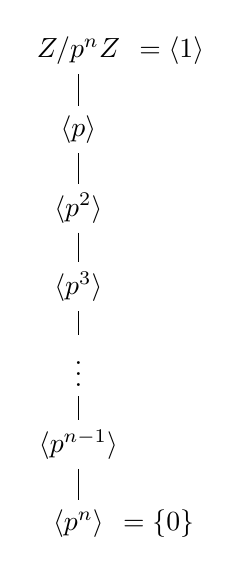
\begin{tikzpicture}[scale=1]
\node (top) at (0,6) {$\mathbb Z/p^n\mathbb Z$};
\node[anchor=west] at (top.east) {$=\langle 1\rangle$};

\node (a1) at (0,5) {$\langle p\rangle$};
\node (a2) at (0,4) {$\langle p^2\rangle$};
\node (a3) at (0,3) {$\langle p^3\rangle$};
\node (dot) at (0,2) {$\vdots$};
\node (an1) at (0,1) {$\langle p^{n-1}\rangle$};

\node (bot) at (0,0) {$\langle p^n\rangle$};
\node[anchor=west] at (bot.east) {$=\{0\}$};

\draw (top.south)--(a1.north);
\draw (a1.south)--(a2.north);
\draw (a2.south)--(a3.north);
\draw (a3.south)--(dot.north);
\draw (dot.south)--(an1.north);
\draw (an1.south)--(bot.north);
\end{tikzpicture}
\end{center}


\item \textbf{克莱因四元群}（Viergruppe）\(V_4\) 是 4 阶群，其乘法表为

\begin{center}
\begin{minipage}[c]{0.35\textwidth}
\centering
$\begin{array}{c|cccc}
\cdot & 1 & a & b & c \\
\hline
1 & 1 & a & b & c \\
a & a & 1 & c & b \\
b & b & c & 1 & a \\
c & c & b & a & 1
\end{array}$
\end{minipage}
\quad 以及格 \quad
\begin{minipage}[c]{0.35\textwidth}
\centering
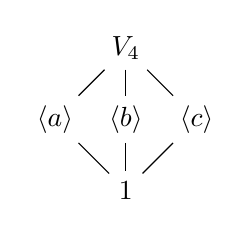
\begin{tikzpicture}[scale=0.9]
% 节点定义
\node (top) at (0,2) {$V_4$};
\node (ha) at (-1,1) {$\langle a\rangle$};
\node (hb) at (0,1) {$\langle b\rangle$};
\node (hc) at (1,1) {$\langle c\rangle$};
\node (bot) at (0,0) {$1$};
% 连线
\draw (top)--(ha);
\draw (top)--(hb);
\draw (top)--(hc);
\draw (ha)--(bot);
\draw (hb)--(bot);
\draw (hc)--(bot);
\end{tikzpicture}
\end{minipage}
\end{center}

注意 \(V_4\) 是阿贝尔群且不同构于 \(Z_4\)（为什么？）。我们将会看到 \(D_8\) 有一个同构于 \(V_4\) 的子群，因此不必验证上述二元运算满足结合律。

\item \(S_3\) 的格为

\begin{center}
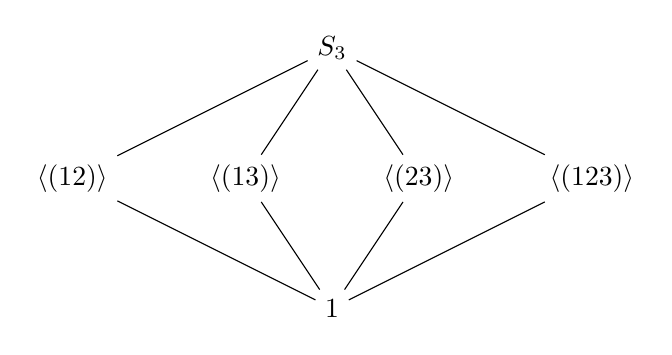
\begin{tikzpicture}[scale=1.1]
%顶层
\node (top) at (2,3) {$S_3$};
%第二层子群
\node (h12) at (-1,1.5) {$\langle(12)\rangle$};
\node (h13) at (1,1.5) {$\langle(13)\rangle$};
\node (h23) at (3,1.5) {$\langle(23)\rangle$};
\node (h123) at (5,1.5) {$\langle(123)\rangle$};
%底层单位元
\node (id) at (2,0) {$1$};

%连线 S3向下
\draw (top)--(h12);
\draw (top)--(h13);
\draw (top)--(h23);
\draw (top)--(h123);

%三个2阶子群连到底元1
\draw (h12)--(id);
\draw (h13)--(id);
\draw (h23)--(id);

%⟨(123)⟩连到底元1
\draw (h123)--(id);
\end{tikzpicture}
\end{center}

\item 使用我们通常的记号 \(D_8 = \langle r, s \rangle\)，\(D_8\) 的格为

\begin{center}
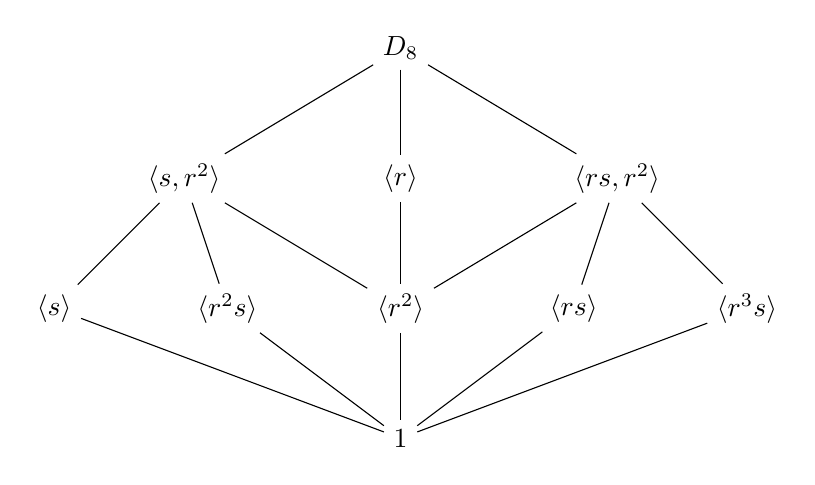
\begin{tikzpicture}[scale=1.1]
% 第1层 顶层
\node (top) at (0,4) {$D_8$};

% 第2层
\node (A) at (-2.5,2.5) {$\langle s,r^2\rangle$};
\node (B) at (0,2.5) {$\langle r\rangle$};
\node (C) at (2.5,2.5) {$\langle rs,r^2\rangle$};

% 第3层
\node (a) at (-4,1) {$\langle s\rangle$};
\node (b) at (-2,1) {$\langle r^2s\rangle$};
\node (c) at (0,1) {$\langle r^2\rangle$};
\node (d) at (2,1) {$\langle rs\rangle$};
\node (e) at (4,1) {$\langle r^3s\rangle$};

% 底层
\node (id) at (0,-0.5) {$1$};

% 顶层连线
\draw (top)--(A);
\draw (top)--(B);
\draw (top)--(C);

% 第二层往下连
\draw (A)--(a);
\draw (A)--(b);
\draw (A)--(c);

\draw (B)--(c);

\draw (C)--(c);
\draw (C)--(d);
\draw (C)--(e);

% 第三层连到底元1
\draw (a)--(id);
\draw (b)--(id);
\draw (c)--(id);
\draw (d)--(id);
\draw (e)--(id);
\end{tikzpicture}
\end{center}


\item \(Q_8\) 的子群格为

\begin{center}
\begin{tikzpicture}[scale=1.1]
%顶层
\node (top) at (0,3) {$Q_8$};
%第二层
\node (i) at (-1.5,1.5) {$\langle i\rangle$};
\node (j) at (0,1.5) {$\langle j\rangle$};
\node (k) at (1.5,1.5) {$\langle k\rangle$};
%第三层
\node (minus1) at (0,0) {$\langle -1\rangle$};
%底层单位元
\node (id) at (0,-1.5) {$1$};

%连线
\draw (top)--(i);
\draw (top)--(j);
\draw (top)--(k);

\draw (i)--(minus1);
\draw (j)--(minus1);
\draw (k)--(minus1);

\draw (minus1)--(id);
\end{tikzpicture}
\end{center}

\item \(D_{16}\) 的格不是平面图（无法在平面上无交叉地画出）。一种画法是

\begin{center}
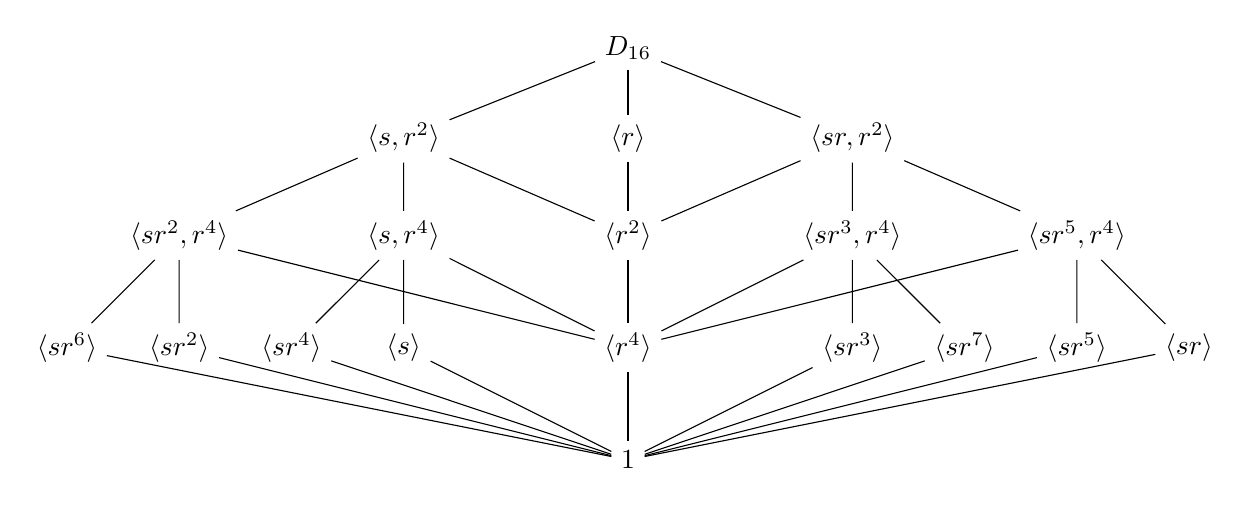
\begin{tikzpicture}[scale=0.95]
% 第1层 顶层 D16
\node (top) at (0,5) {$D_{16}$};

% 第2层
\node (A) at (-3,3.8) {$\langle s,r^2\rangle$};
\node (B) at (0,3.8) {$\langle r\rangle$};
\node (C) at (3,3.8) {$\langle sr,r^2\rangle$};

% 第3层
\node (a) at (-6,2.5) {$\langle sr^2,r^4\rangle$};
\node (b) at (-3,2.5) {$\langle s,r^4\rangle$};
\node (c) at (0,2.5) {$\langle r^2\rangle$};
\node (d) at (3,2.5) {$\langle sr^3,r^4\rangle$};
\node (e) at (6,2.5) {$\langle sr^5,r^4\rangle$};

% 第4层
\node (a1) at (-7.5,1) {$\langle sr^6\rangle$};
\node (a2) at (-6,1) {$\langle sr^2\rangle$};
\node (b1) at (-4.5,1) {$\langle sr^4\rangle$};
\node (b2) at (-3,1) {$\langle s\rangle$};
\node (mid) at (0,1) {$\langle r^4\rangle$};
\node (d1) at (3,1) {$\langle sr^3\rangle$};
\node (d2) at (4.5,1) {$\langle sr^7\rangle$};
\node (e1) at (6,1) {$\langle sr^5\rangle$};
\node (e2) at (7.5,1) {$\langle sr\rangle$};

% 底层 单位元
\node (id) at (0,-0.5) {$1$};

% ========== 连线 ==========
% 顶层 -> 第二层
\draw (top)--(A);
\draw (top)--(B);
\draw (top)--(C);

% 第二层 -> 第三层
\draw (A)--(a);
\draw (A)--(b);
\draw (A)--(c);

\draw (B)--(c);

\draw (C)--(c);
\draw (C)--(d);
\draw (C)--(e);

% 第三层 -> 第四层
\draw (a)--(a1);
\draw (a)--(a2);
\draw (a)--(mid);

\draw (b)--(b1);
\draw (b)--(b2);
\draw (b)--(mid);

\draw (c)--(mid);

\draw (d)--(mid);
\draw (d)--(d1);
\draw (d)--(d2);

\draw (e)--(mid);
\draw (e)--(e1);
\draw (e)--(e2);

% 第四层 -> 底层1
\draw (a1)--(id);
\draw (a2)--(id);
\draw (b1)--(id);
\draw (b2)--(id);
\draw (mid)--(id);
\draw (d1)--(id);
\draw (d2)--(id);
\draw (e1)--(id);
\draw (e2)--(id);
\end{tikzpicture}
\end{center}

\end{enumerate}
\end{example}


在许多理论证明和具体例子中，我们只关心给定群的两个（或少数几个）子群及其相互关系。为了图形化地描绘这些，我们将画出整个群格的一个\textbf{子格}，其中包含相关的并与交。在这样的子格中，一条无中断的线通常并不意味着线的端点之间没有子群。这些部分格也用于处理无限群。例如，如果我们只想讨论 \(D_{16}\) 的子群 \(\langle sr^2, r^4 \rangle\) 和 \(\langle r^2 \rangle\) 之间的关系，我们会画出子格

\begin{center}
\begin{tikzpicture}[scale=1.1]
%第一层
\node (top) at (0,4) {$D_{16}$};
%第二层
\node (A) at (0,2.8) {$\langle s,r^2\rangle$};
%第三层
\node (B) at (-1.8,1.6) {$\langle sr^2,r^4\rangle$};
\node (C) at (1.8,1.6) {$\langle r^2\rangle$};
%第四层
\node (D) at (0,0.4) {$\langle r^4\rangle$};
%底层
\node (id) at (0,-0.8) {$1$};

\draw (top)--(A);
\draw (A)--(B);
\draw (A)--(C);
\draw (B)--(D);
\draw (C)--(D);
\draw (D)--(id);
\end{tikzpicture}
\end{center}
注意 \(\langle s, r^2 \rangle\) 和 \(\langle r^4 \rangle\) 分别是这两个子群在 \(D_{16}\) 中的并和交。

最后，给定群的子群格，计算正规化子和中心化子相对容易。例如，在 \(D_8\) 中我们可以看出 \(C_{D_8}(s) = \langle s, r^2 \rangle\)，因为我们首先计算 \(r^2 \in C_{D_8}(s)\)（见第 2 节）。这证明了 \(\langle s, r^2 \rangle \leq C_{D_8}(s)\)（注意元素总是属于它自己的中心化子）。包含 \(\langle s, r^2 \rangle\) 的子群只有该子群本身和整个 \(D_8\)。不能有 \(C_{D_8}(s) = D_8\)，因为 \(r\) 不与 \(s\) 可交换（即 \(r \notin C_{D_8}(s)\)）。因此只剩下所声称的 \(C_{D_8}(s)\) 的可能性。

\subsection*{习题}

\begin{enumerate}[label=\arabic*]
\item 设 \(H\) 和 \(K\) 是 \(G\) 的子群。画出所有可能只显示 \(G, 1, H, K\) 及其并和交的子格。不同的画法有什么区别？

\item 在 (a) 到 (d) 中列出 \(D_{16}\) 中满足给定条件的所有子群。
\begin{enumerate}[label=(\alph*)]
\item 包含在 \(\langle sr^2, r^4 \rangle\) 中的子群；
\item 包含在 \(\langle sr^7, r^4 \rangle\) 中的子群；
\item 包含 \(\langle r^4 \rangle\) 的子群；
\item 包含 \(\langle s \rangle\) 的子群。
\end{enumerate}

\item 证明 \(D_8\) 的子群 \(\langle s, r^2 \rangle\) 同构于 \(V_4\).

\item 利用给出的格找出所有生成 \(D_8\) 的元素对（共有 12 对）。

\item 利用给出的格找出所有 \(x \in D_{16}\) 使得 \(D_{16} = \langle x, s \rangle\)（共有 16 个这样的 \(x\)）。

\item 利用给出的格帮助找出下列群中每个元素的中心化子：
\begin{enumerate}[label=(\alph*)]
\item \(D_8\)；
\item \(Q_8\)；
\item \(S_3\)；
\item \(D_{16}\)。
\end{enumerate}

\item 求 \(D_{16}\) 的中心。

\item 在下列群中，求每个子群的正规化子：
\begin{enumerate}[label=(\alph*)]
\item \(S_3\)；
\item \(Q_8\)。
\end{enumerate}

\item 画出下列群的子群格：
\begin{enumerate}[label=(\alph*)]
\item \(\mathbb{Z}/16\mathbb{Z}\)；
\item \(\mathbb{Z}/24\mathbb{Z}\)；
\item \(\mathbb{Z}/48\mathbb{Z}\)。[见第 3 节习题 6。]
\end{enumerate}

\item 通过证明若 \(|G| = 4\) 则 \(G \cong Z_4\) 或 \(G \cong V_4\) 来分类 4 阶群。[见第 1.1 节习题 36。]

\item 考虑如下表示的 16 阶群：
\[
QD_{16} = \langle \sigma, \tau \mid \sigma^8 = \tau^2 = 1,\ \sigma \tau = \tau \sigma^3 \rangle
\]
（称为 16 阶拟二面体群或半二面体群）。该群有三个 8 阶子群：\(\langle \tau, \sigma^2 \rangle \cong D_8\)，\(\langle \sigma \rangle \cong Z_8\) 和 \(\langle \sigma^2, \sigma \tau \rangle \cong Q_8\)，并且每个真子群都包含在这三个子群之一中。在下页的拟二面体群的所有子群格中填入缺失的子群，每个子群用至多两个生成元表示。（这是另一个非平面格的例子。）

接下来的三个例子引出两个不同构但具有相同子群格的群。

\item 群 \(A = Z_2 \times Z_4 = \langle a, b \mid a^2 = b^4 = 1,\ ab = ba \rangle\) 的阶为 8，有三个 4 阶子群：\(\langle a, b^2 \rangle \cong V_4\)，\(\langle b \rangle \cong Z_4\) 和 \(\langle ab \rangle \cong Z_4\)，并且每个真子群都包含在这三个子群之一中。画出 \(A\) 的所有子群格，每个子群用至多两个生成元表示。

\begin{center}
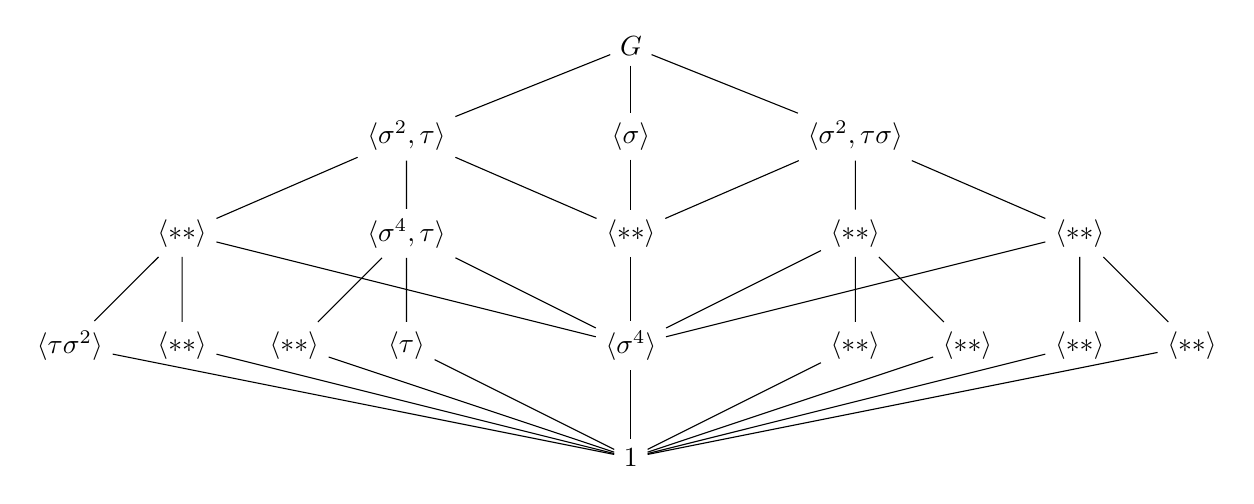
\begin{tikzpicture}[scale=0.95]
% 第1层 顶层 G
\node (top) at (0,5) {$G$};

% 第2层
\node (A) at (-3,3.8) {$\langle \sigma^2,\tau\rangle$};
\node (B) at (0,3.8) {$\langle \sigma\rangle$};
\node (C) at (3,3.8) {$\langle \sigma^2,\tau\sigma\rangle$};

% 第3层
\node (a) at (-6,2.5) {$\langle{**}\rangle$};
\node (b) at (-3,2.5) {$\langle \sigma^4,\tau\rangle$};
\node (c) at (0,2.5) {$\langle{**}\rangle$};
\node (d) at (3,2.5) {$\langle{**}\rangle$};
\node (e) at (6,2.5) {$\langle{**}\rangle$};

% 第4层
\node (a1) at (-7.5,1) {$\langle \tau\sigma^2\rangle$};
\node (a2) at (-6,1) {$\langle{**}\rangle$};
\node (b1) at (-4.5,1) {$\langle{**}\rangle$};
\node (b2) at (-3,1) {$\langle \tau\rangle$};
\node (mid) at (0,1) {$\langle \sigma^4\rangle$};
\node (d1) at (3,1) {$\langle{**}\rangle$};
\node (d2) at (4.5,1) {$\langle{**}\rangle$};
\node (e1) at (6,1) {$\langle{**}\rangle$};
\node (e2) at (7.5,1) {$\langle{**}\rangle$};

% 底层 单位元
\node (id) at (0,-0.5) {$1$};

% ========== 连线 ==========
% 顶层 -> 第二层
\draw (top)--(A);
\draw (top)--(B);
\draw (top)--(C);

% 第二层 -> 第三层
\draw (A)--(a);
\draw (A)--(b);
\draw (A)--(c);

\draw (B)--(c);

\draw (C)--(c);
\draw (C)--(d);
\draw (C)--(e);

% 第三层 -> 第四层
\draw (a)--(a1);
\draw (a)--(a2);
\draw (a)--(mid);

\draw (b)--(b1);
\draw (b)--(b2);
\draw (b)--(mid);

\draw (c)--(mid);

\draw (d)--(mid);
\draw (d)--(d1);
\draw (d)--(d2);

\draw (e)--(mid);
\draw (e)--(e1);
\draw (e)--(e2);

% 第四层 -> 底层1
\draw (a1)--(id);
\draw (a2)--(id);
\draw (b1)--(id);
\draw (b2)--(id);
\draw (mid)--(id);
\draw (d1)--(id);
\draw (d2)--(id);
\draw (e1)--(id);
\draw (e2)--(id);
\end{tikzpicture}
\end{center}


\item 群 \(G = Z_2 \times Z_8 = \langle x, y \mid x^2 = y^8 = 1,\ xy = yx \rangle\) 的阶为 16，有三个 8 阶子群：\(\langle x, y^2 \rangle \cong Z_2 \times Z_4\)，\(\langle y \rangle \cong Z_8\) 和 \(\langle xy \rangle \cong Z_8\)，并且每个真子群都包含在这三个子群之一中。画出 \(G\) 的所有子群格，每个子群用至多两个生成元表示（见习题 12）。

\item 设 \(M\) 是具有如下表示的 16 阶群：
\[
\langle u, v \mid u^2 = v^8 = 1,\ vu = uv^5 \rangle
\]
（有时称为 16 阶模群）。它有三个 8 阶子群：\(\langle u, v^2 \rangle\)，\(\langle v \rangle\) 和 \(\langle uv \rangle\)，并且每个真子群都包含在这三个子群之一中。证明 \(\langle u, v^2 \rangle \cong Z_2 \times Z_4\)，\(\langle v \rangle \cong Z_8\) 和 \(\langle uv \rangle \cong Z_8\)。证明 \(M\) 的子群格与 \(Z_2 \times Z_8\) 的子群格相同（见习题 13），但这两个群不同构。

\item 描述 \(D_{16}\) 的三个 8 阶子群各自的同构类型。

\item 利用 16 阶拟二面体群的子群格证明，每个 2 阶元都包含在真子群 \(\langle \tau, \sigma^2 \rangle\) 中（见习题 11）。

\item 利用 16 阶模群 \(M\) 的子群格证明，集合 \(\{x \in M \mid x^2 = 1\}\) 是 \(M\) 的一个子群，同构于克莱因四元群（见习题 14）。

\item 利用子群格帮助找出 \(QD_{16}\) 中每个元素的中心化子（见习题 11）。

\item 利用子群格帮助找出 \(N_{D_{16}}(\langle s, r^4 \rangle)\)。

\item 利用 \(QD_{16}\) 的子群格（见习题 11）帮助找出下列正规化子：
\begin{enumerate}[label=(\alph*)]
\item \(N_{QD_{16}}(\langle \tau \sigma \rangle)\)；
\item \(N_{QD_{16}}(\langle \tau, \sigma^4 \rangle)\)。
\end{enumerate}
\end{enumerate}